% !TEX encoding = IsoLatin



%%%%%%%%%%%%%%%%%%%%%%%%%%%%%%%%%%%%%%%%%%%%%%%%%%%% 1.o Esempio con la classe toptesi
\documentclass[b5paper,10pt,twoside,cucitura]{toptesi}
\usepackage{lipsum}
%\documentclass[twoside,cucitura,pdfa]{toptesi}
%%%%%%%%%%%%%%%%%%%%%%%%%%%%%%%%%%%%%%%%%%%%%%%%%%%% 2.o Esempio con la classe toptesi
% \documentclass[11pt,twoside,oldstyle,autoretitolo,classica,greek]{toptesi}
% \usepackage[or]{teubner}
%%%%%%%%%%%%%%%%%%%%%%%%%%%%%%%%%%%%%%%%%%%%%%%%%%%%
% Commentare la riga seguente se si � specificata l'opzione "pdfa"
\usepackage{hyperref}
\usepackage{graphicx}
\usepackage{url}
\usepackage{natbib} 



\graphicspath{ {images/} }

\hypersetup{%
    pdfpagemode={UseOutlines},
    bookmarksopen,
    pdfstartview={FitH},
    colorlinks,
    linkcolor={blue},
    citecolor={red},
    urlcolor={blue}
  }
%
% Esempio di composizione di tesi di laurea con PDFLATEX <---------------- !
%
% Questo esempio e' stato preparato inizialmente il 13-marzo-1989
% e poi e' stato modificato via via che TOPtesi andava
% arricchendosi di altre possibilit�.
%
% Per comporre con XeLaTeX, invece che con pdfLaTeX, vedere il file
% toptesi-example-xetex.tex
% A parteIfont, bisogna specificare alcune cose dopo la fine del preambolo.
%
% Nel seguito laurea "quinquennale" sta anche per "specialistica" o "magistrale".
%
% Cambiare encoding a piacere; oppure non caricare nessun encoding se si usano
% solo caratteri a 7 bit (ASCII) nei file d'entrata. La codifica utf8 sarebbe
% quella maggiormente desiderabile; richiede per� un editor che sappia gestirla.
%
\usepackage[utf8]{inputenc}% per macchine Linux/Mac/UNIX/Windows; meglio utf8
\usepackage[T1]{fontenc}\usepackage{lmodern}
%
\ateneo{Politecnico di Torino}
\nomeateneo{}
\FacoltaDi{}
\facolta[III]{}
%\Materia{Remote sensing}
%\monografia{La pressione barometrica di Giove}% per la laurea triennale
\titolo{Multi-channel Conversational Agent for Personalized Music Recommendations}% per la laurea quinquennale e il dottorato
\sottotitolo{}% per la laurea quinquennale e il dottorato
\corsodilaurea{Computer Science}% per la laurea
%\corsodidottorato{Meccanica}% per il dottorato

%%%%%%% Trucco per inserire la matricola sotto il nome di ogni candidato
\candidato{\tabular{@{}l@{}}Giulio \textsc{Verazzo}\\matricola: 225208\endtabular}% per tutti I percorsi


%%%%%%% 
%\direttore{prof. Albert Einstein}% per il dottorato
%\coordinatore{prof. Albert Einstein}% per il dottorato
\relatore{prof.\ Maurizio Morisio}% per la laurea e/o il dottorato


\tutoreaziendale{dott.\ ing.\ Giuseppe Rizzo}

%\sedutadilaurea{Agosto 1615}% per la laurea quinquennale; oppure:
\sedutadilaurea{\textsc{Anno~accademico} 2017-2018}% per la laurea magistrale
%\esamedidottorato{Novembre 1610}% per il dottorato
%\annoaccademico{1615-1616}% solo con l'opzione classica
%\annoaccademico{2006-2007}% idem
\ciclodidottorato{XV}% per il dottorato
%\logosede{logotrieste}% questo e' ovviamente facoltativo, ma e' richiesto per
% il dottorato al PoliTO; in questo calso si usa il "logopolito"
\logosede{lion} % auxiliary ShareLaTeX logo
%
%\chapterbib %solo per vedere che cosa succede; e' preferibile comporre una sola bibliografia
%\AdvisorName{Supervisors}
\newtheorem{osservazione}{Osservazione}% Standard LaTeX

%\setbindingcorrection{3mm}

\begin{document}\errorcontextlines=9% debugging

\english%  di default vale \italiano

% Comment the following lines if you don't care about the title page in English
% Change the strings if you want a title page and a copyright page in another language
% Comment just the \iflanguage statement and the closing line of the language test
%	 if you want to make a global change instead of a conditional one.
%%%%%%%%%%%%%%%%%%%%%%%%%%%%%%%%%%%%%%%%%
	\iflanguage{english}{%
	\retrofrontespizio{This work is subject to the Creative Commons Licence}
	\DottoratoIn{PhD Course in\space}
	\CorsoDiLaureaIn{Master degree course in\space}
	\NomeMonografia{Bachelor Degree Thesis}
	\TesiDiLaurea{Master Degree Thesis}
	\NomeDissertazione{PhD Dissertation}
	\InName{in}
	\CandidateName{Candidate}% or Candidate
	\AdvisorName{Supervisor}% or Supervisor
	\TutorName{Tutor}
	\NomeTutoreAziendale{Internship Tutor}
	\CycleName{cycle}
	\NomePrimoTomo{First volume}
	\NomeSecondoTomo{Second Volume}
	\NomeTerzoTomo{Third Volume}
	\NomeQuartoTomo{Fourth Volume}
	\logosede{logopolito}% or comma separated list of logos
	\sedutadilaurea{\textsc{Academic~Year} 2017-2018}% per la laurea magistrale
	}{}
%%%%%%%%%%%%%%%%%%%%%%%%%%%%%%%%%%%%%%%%%

\expandafter\ifx\csname StileTrieste\endcsname\relax
    \frontespizio
\else
    \paginavuota
    \begin{dedica}
        A mio padre

        \textdagger\ A mio nonno Pino
    \end{dedica}
    \tomo
\fi

\ringraziamenti



\indici

\mainmatter


\chapter{Introduction}

Recent technological advances in entertainment applications all moves in the direction of providing the user with an increasingly tailor-made and personalized experience. The reasons for this phenomenon are to be found in the need of the main platforms, to offer quality content and above all, relevant to each user in order to increase the engagement and improve the overall experience (and therefore revenues). The amount of data available is enormous and the development of intelligent and automatic filters is one of the main technological challenges currently underway. In this panorama, different actors are moving, such as recommender systems, chatbots and applications for affective computing. The aim of this thesis work is to explore and evaluate, in terms of design, usability and usefulness, the use of a conversational interface for a recommender system, whose input data are previously filtered through an affective computing software. In detail, the application developed is a multi-platform chatbot, named \textit{Beat in a Bot}, whose purpose is to recommend music artists to listen, based on musical genres preferences shared among groups of people with the same personality. The result is a complete and usable product, currently available to the public on Telegram and Facebook Messenger platforms. The work is presented as follows: the first chapter contains an overview on the background of all the pieces of the project. The second chapter includes first a description of the high-level architecture and then the details of every single component. The third chapter is dedicated to the implementation  and explains all the technical aspects of the application. The fourth chapter shows the results of the evaluation process composed by the design, usability and usefulness test. The last chapter is about future improvements and possibility of monetization of the product. 

\chapter{Background}

\section{Chatbots}
\subsection{Introduction}
Messaging platforms plays a big role in today's communications as shown by the 18.7 billion text messages sent everyday. Text messages are fast, easy to use, cheap or almost free, can be used in formal or informal contexts, they aren't intrusive like a phone call and they can be ubiquitous; we can send them from desktop or mobile systems like smartphones, tablets and smartwatches. All these things explains why text messages are so popular globally and why messaging platforms are growing exponentially in terms off app usage and time spent.
A chatbot could be thought as someone to chat with, that is always available and will answer to all the questions in his sphere of understanding with the only exception that he is not human. From a technical perspective, a chatbot is a computer program which conducts a conversation via auditory or textual methods with the intention of simulating a human-like behaviour   \citep{techtarget}. Chatbots are part of the instant messaging world, that are applications where one feels more connected with individuals while communicating textually.
Instant messaging apps like chatbots uses WebSocket or other real-time communication protocols which provide the reliability and speed required for real-time text transmission. There is a big variety of chatbot applications, from ones that can handle few questions based on keywords for few tasks, to ones that uses Natural Language Processing and Artificial Intelligence, able to learn from his interlocutor to improve himself over time.


\begin{figure}[h]
\centering 
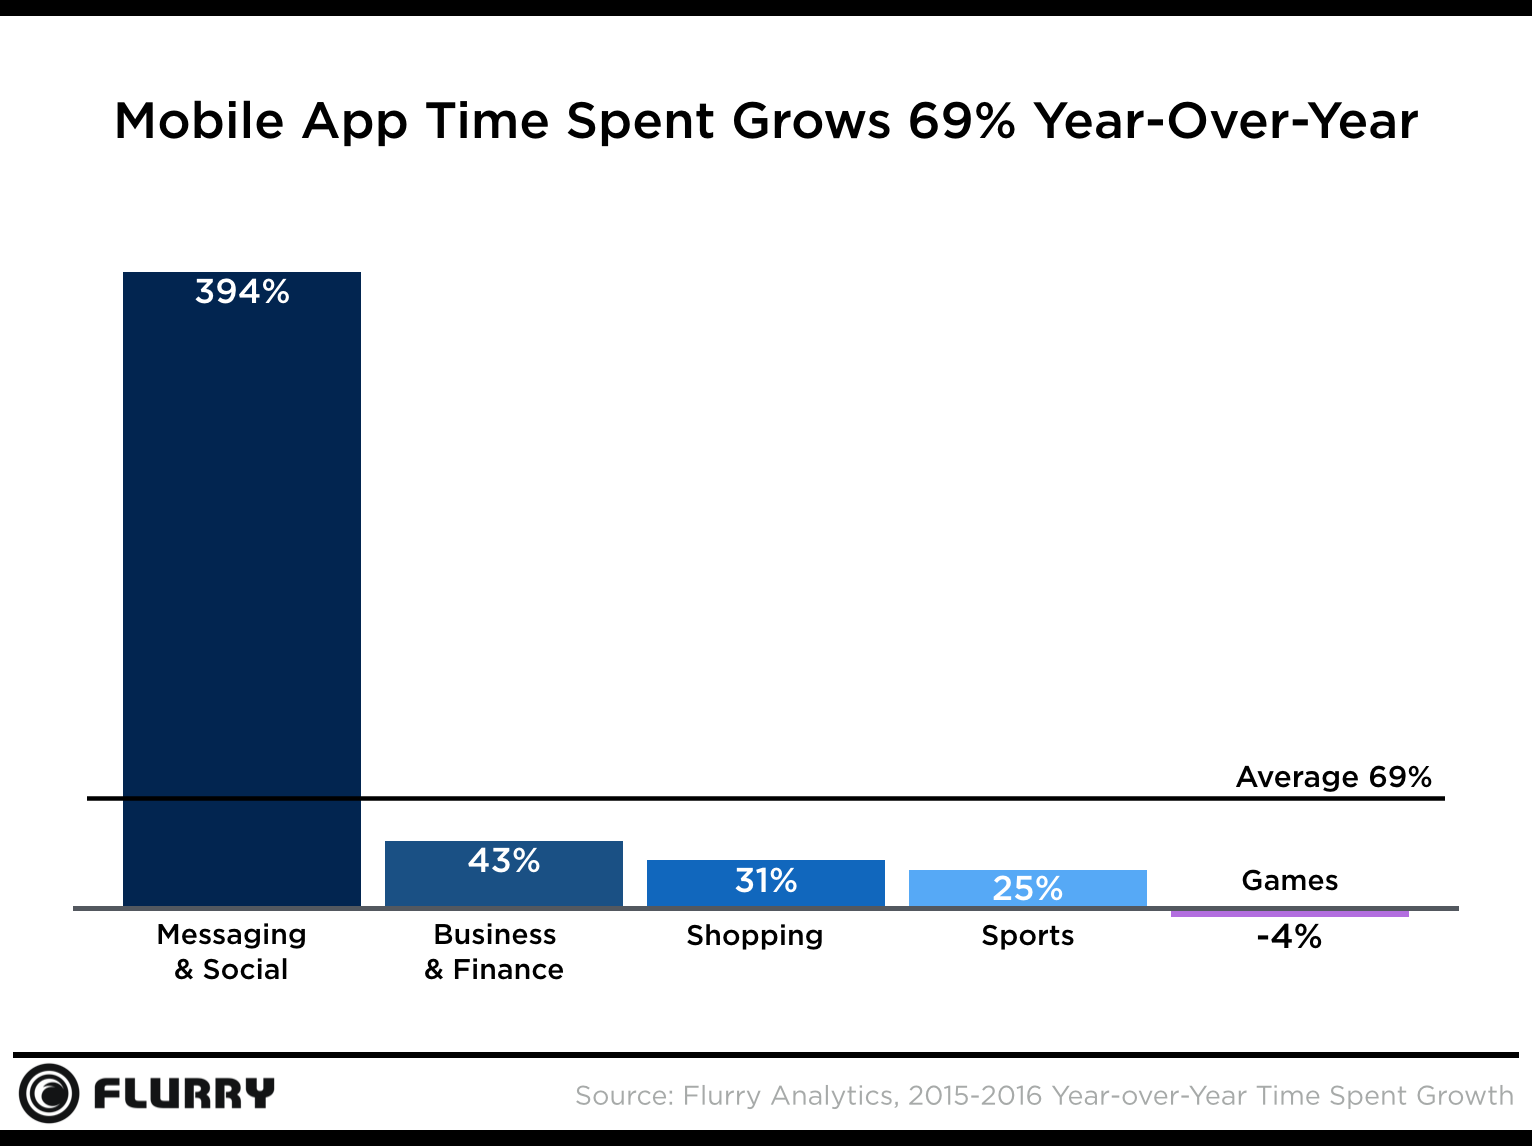
\includegraphics[width=\textwidth]{time_spent.png}
\caption{Flurry Analytics, 2015–2016 Year-Over-Year Time Spent Growth.}
\end{figure}


\subsection{History of chatbots}

The first evidence of this kind of computer programs comes from Alan Turing, an Englishman known as the father of computer science, who was a computer scientist, cryptanalyst, logician and mathematician. In 1950 he published his famous article \textit{Computing Machinery and Intelligence}  \citep{turing} which is used nowadays as the basis of intelligence assessment of computer programs. In this article, he proposed a criteria to determine if a machine is able to think or not; this is known as the \textit{Turing Test} and depends on the ability of a computer program to impersonate a human in a real-time written conversation with a human judge, sufficiently well that the judge is unable to distinguish, reliably on the basis of the conversational content alone, between the program and a real human. 
The criteria of Alan Turing inspired Joseph Weizenbaum, a German-American computer scientist and professor at Massachusetts Institute of Technology, who in 1966 published a program called ELIZA  \citep{eliza}. The ELIZA program was built with the purpose to give to his interlocutor, an illusion of intelligence, making people to think they were talking to a real human. His algorithm (used by all the chatbot makers) was able to analyze the input given by the users by searching from phrases and keywords, and give pre-planned responses. For instance, given a sentence ELIZA would do the following in order:

\begin{itemize}
    \item 
    Receive the input and store them in memory for further analysis
    \item 
    Search for keywords in the sentence
    \item 
    Give back the pre-programmed response if a keyword is matched
    \item 
    Give back the default answer "Sorry, don't know about that" if there is no clear match.
\end{itemize}

So, in a sentence containing the keyword "mother" a typical response by ELIZA would be "Tell me more about your family". Although the simplicity of the algorithm, this was enough to give an illusion of intelligence to a human judge showing the fact that such an illusion is  surprisingly easy to generate, because humans are so ready to give the benefit of the doubt when conversational responses are likely to be interpreted as "intelligent".
The term "ChatterBot", that became then "chatbot" in the literature to follow, was coined in 1994 by Michael Mauldin, an American inventor and scientist, founder of Lycos Inc., who created the program Verbot, a popular chatbot who followed the path traced by ELIZA. Its latest version called Sylvie, can be considered as the first intelligent animated virtual human: it incorporates real-time animation as well as speech and natural language processing. The idea was to develop a conversational agent that could act as a human-machine interface. Thanks to the latest progress in the field of Artificial Intelligence, chatbots can develop their skills and learn with every single chat. So, the more conversations about different topics they have, the more skilled they become. Such a chatbot doesn't get stuck when he gets unknown questions because he can quickly make connections between various notions and come to an answer. A good example of a chatbot power by artificial intelligence is Cleverbot  \citep{cleverbot} created by British AI scientist Rollo Carpenter. Cleverbot uses artificial intelligence to learn from human inputs in order to give responses that are not pre-programmed. It responds to the input by finding how a human responded to that input when it was asked. Cleverbot has reached a score of 59.3\% to the Turing Test, compared to the rating of 63.3\% human achieved by human participants. A score of 50.05\% or higher is often considered to be a passing grade  \citep{jacob}. The introduction of artificial intelligence in the field of conversational agents, has attracted the attention of the big companies of the IT world, which have started to release commercial products that use this technology. Apple started the trend with the introduction of Siri, the first digital smartphone assistant, followed by products such as Amazon's Alexa, Google Assistant, Microsoft's Cortana and Samsung's Bixby to citep the most popular. Their most common features are: send text and emails, make phone calls, schedule appointments, check the weather, stocks and flight status, make conversions and translations, search on the web, find what song is playing the room, buy products on online stores, tells you when to leave based on the expected traffic and more. The interest of such big companies to the digital assistants world, is a sign of the enormous potential of this technology and how much it will havean impact it the future of our lives. 

\subsection{Types of chatbots}

Chatbot can be grouped in three big categories: mimicry bots, intent-based bots and conversational agents. 

\subsubsection{Mimicry bots}

These bots doesn't have the concept of statement meaning. They only provide an appearance of conversation without understanding what is being said. These bots can be rather simple like rule-based model bots or powered by Artificial Intelligence like sequence-to-sequence bots. 
\\
Rule-based model bot working logic is as follows:
the developer writes a \textit{pattern} and a \textit{template}; when the bot encounters that pattern in a sentence from user, it replies with one of the templates. Those kind of bots are easy to create but it is incredibly difficult to make them answer to complex queries. The pattern matching is weak and hence, time consuming and takes a lot of effort to write the rules manually. A good example of this kind of bots is ELIZA. ELIZA consisted of a simple substitution rules to mimic a psychologist from 1960s. The main idea was that the bot simply replies to the questions by repeating back the words of the questioner. If the question was "should I buy an orange?" a possible answer was "tell me why you should buy an orange". 
\\
Sequence-to-sequence based bots instead, uses deep learning to learn from example conversations. They train on a bunch of dialogs and learn to generate the next statement given the last statement. Lots of dialogs dataset can be found on the internet like OpenSubtitles, Ubuntu Dialog Corpus or replies to tweets from Twitter.
A sequence-to-sequence model consists of an encoder and a decoder. Both are implemented using recurrent neural networks. The encoder takes as input a set of words (called "tokens") and generates a vector that goes as input into the decoder which generates a set of tokens until it generates a special stop symbol. This approach is vastly used in language translation. A set of italian words like "il libro {\`e} sul tavolo" is transformed into a vector and translated into "the book is on the table" thanks to the number of learning sessions the machine has done. Conversation can be seen as a translation if we substitute the source language with the question and the destination language with the answer.
The problem with sequence-to-sequence models is that they are devoid of meaning, the bot does not have any knowledge of the world. For instance, in the statement "buy me 3 apples" there is no difference between 3 apples or 300 for the machine and this may cause understanding and evaluating problems.
Intelligent models can learn from existing human conversations. They can be classified into:

\begin{enumerate}
    \item Retrieval-based models
    \item Generative models
\end{enumerate}

Retrieval-based models pick a response from a collection of responses based on the query. Since it does not generate any new sentences, we don't need to worry about the grammar.
The Generative models instead, generate responses word by word and, due to this, the responses are prone to grammatical errors. These models are difficult to train as they need to learn the proper sentence structure by themselves. However, once trained, the generative models outperforms any other model in terms of speak quality and they can also handle unseen queries.

\subsubsection{Intent-based bots}
Bots from this category can provide real conversation but they can't switch between multiple topics. These agents understand language as commands and they use that understanding to perform tasks in the world. Siri, Cortana, Amazon Alexa and Google Home are examples of intention-based agents.
The understanding is divided into two subproblems:
\begin{itemize}
    \item Identifying what the user wants the machine to do (the "intent").
    \item Figuring out the details of the intent.
\end{itemize}
For example, if we ask our assistant to "Play Jazz", it first needs to understand that we wanna play music (the intent) and then it must understand that, in particular, we want to hear Jazz music (the details).
Intent can be understood in many ways, using keywords, with text-based classification or with deep learning and Convolutional Neural Networks. To use keywords, simply associate words and phrases with intents. To do text-based classification, a bunch of statements must be labeled with the correct intent and then a classifier must be trained over them. 
Once the agent has determined the intent, it needs to convert the statement into a machine readable form. This conversion is made possible thanks to Natural Language Understanding techniques such as word embeddings \citep{wordembeddings}, which converts words or phrases into vectors of real numbers so that they can be manipulated by NLP algorithms.

\subsubsection{Conversational Agents}

Those are expansion of Intent-based agents to add multi-turn conversation. This is done by keeping track of the state of the conversation and knowing when the person wants to talk about something else. A good implementation of this concept is the framework RavenClaw  \citep{ravenclaw} which uses a dialog stack and an expectation agenda. The dialog stack keeps track of all the thing the chatbot wants to talk about. The expectation agenda is a data structure to keep track of what the chatbot expects to hear.
For example, the chatbot asks, "what is 4+5?"; on the top of the dialog stack there is the 4+5 question and the expectation agenda is filled with the answer "9". Let's say the user replies "buy me a pizza", the bot needs to switch the context of the conversation and so, the dialog stack is pushed with "order groceries" and the expectation agenda is updated with possible answers and questions about ordering food.
Another possible implementation can be done using a machine learning approach with reinforcement learning. Reinforcement learning consists of a set of states, actions and a reward function that provides a reward for being in a state s and taking an action a. The idea is that the chatbot has states made of what the bot knows (questions it has answered), the last thing the bot said and the last thing the user said. The bot has to learn a policy (a rule) that gives the best action a for being in state s. 
The problem is that learning a policy requires a lot of training and also, it hard to know exactly what state the agent is because of errors in speech-to-text or errors in understanding.


\subsection{Current state of chatbots and limitations}

The growing interest in chatbots can be explained viewing at three different perspectives.
From a financial perspective, business owners realized the usefulness chatbots can provide to end users, especially when the information can be categorized into concrete and predictable subjects. For example, chatbots can be easily integrated into the customer support experience making the company available to users 24 hours 7 days a week. In addition to that, it is proven that customers prefer to chat with a fast responding customer support rather than find the number and wait to the phone until their turn to come. A chatbot can easily handle all the Frequently Asked Question and when the problem cannot be solved by the machine, he could refer the users to the appropriate technician that is now freed from the hassle of repeating again the same things over and over. This is also good to separate the mechanic work from the brain work giving the machine and the human the jobs that suits them well both. From a user perspective, chatbots can finally give them the best interface to a machine for the human: the word, written or spoken. This opens to a whole new world of possibilities, users can now speak to a machine asking for the information they are searching for, in the most natural way.
From a development perspective, big companies has announced and released their Software Development Kits and Application Programming Interfaces giving the developers the ability to make their own chatbot available for the users: Apple with his iPhone assistant Siri, IBM with the Watson project, Google with Google Home, Amazon with Echo, Microsoft with Cortana, Facebook with the Messenger platform and many others.
Bots are able to understand the intent of the user relatively well only if the interface is made of a set of pre-defined commands hidden in keywords. Problems come to rise when they have to fully understand human language. 

Chatbots today are facing those main problems:

\begin{itemize}
\item They cannot negotiate meanings
\item They can't experience human feelings
\item They have problems with prosody (the way phrases are pronounced)
\item They have problems with logical inference (make a logical assumption given what is been said).
\end{itemize}

When we refer to an object, the agent has never held the object or used it so it will have a limited understanding of it. Since meanings that chatbots have are largely fixed we currently can't negotiate meaning with them.
In conclusion, the state of art is that we can build knowledge into chatbot that they can use to cooperate with us on tasks requiring minimal understanding. Building better chatbots will necessitate knowledge engineering and research into how agents can better follow and adapt to the subtleties of meaning and conversation.

\newpage

\section{Recommender systems}

\subsection{Introduction}
On the Internet, where the number of choices is overwhelming, there is need to filter, prioritize and efficiently deliver relevant information in order to alleviate the problem of information overload, which has created a potential problem to many Internet users. Recommender systems solve this problem by searching through large volume of dynamically generated information to provide users with personalized content and services.
In this chapter, there will be a section about what is a recommender system and how it works, from a more general perspective to technical one. There will be a section about why recommender systems are becoming so popular nowadays, another section showings the different algorithms of recommender systems and finally what it the current state of the art as well as what are the limitations and the challenges we have to face.

\subsection{Fundamentals of recommender systems}

Recommender systems are information filtering systems that deal with the problem of information overload by filtering vital information fragment out of large amount of dynamically generated information according to user's preferences, interests, or observed behavior over time. Recommender systems are used today for large variety of tasks and can be beneficial to both service providers and users. They reduce transaction costs of finding and selecting items in an online shopping environment and it is proven that they can improve the decision making process and quality: showing users items that might interest them, increases the time spent on the platform and therefore the likelihood of a purchase being made. In scientific libraries, recommender systems support users by allowing them to move beyond catalog searches. From a technical perspective, they are computer algorithms that uses linear algebra theorems to predicts a user preference from a user-item matrix so, to implement a recommender system, a \textit{user-item} matrix is first needed. Such matrix has all the users on the rows and all the items on the columns. Each value of the matrix can be the rating that a particular user gave to a particular item. Obviously, users have rated only a limited number of items and so the matrix is sparse. This brings us to the goal of the algorithm that is, to fill all the empty boxes with the predicted ratings for the users to the items. The way the user-item matrix is filled, depends on the typology of recommender systems which are presented in the following section.

\begin{figure}[h]
\centering 
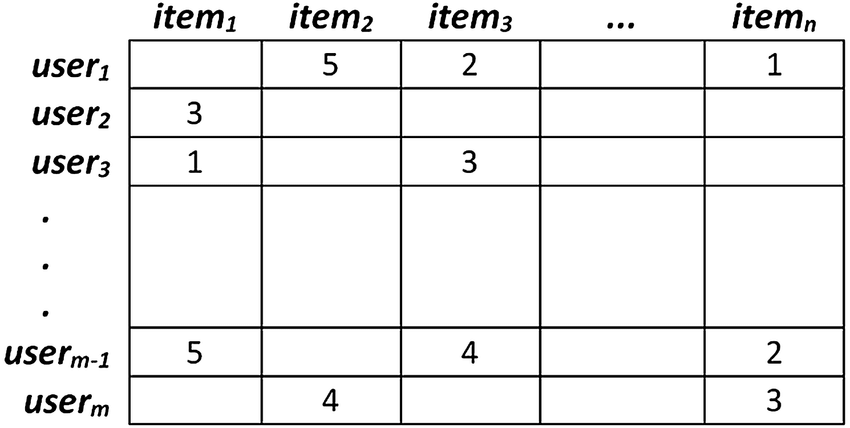
\includegraphics[scale=0.3]{user-item_matrix}
\caption{An example of user-item matrix}
\end{figure}
 
 
\subsection{Types of recommender systems}

Since recommender systems can be used in a large variety of applications, different types of algorithms have been developed each with its peculiarities, pros and cons. Recommender system algorithms can be divided into, Content-based filtering, Collaborative filtering and Hybrid filtering.

\subsubsection{Content-based filtering}

Content-based filtering algorithm main idea is based on the concept that two items are similar if their characteristics are also similar. For instance, two pair of shoes are considered similar if they are of the same brand or belongs to the same category, let's say boots. Usually this type of filtering is used with text documents like books or articles. Items are represented in terms of descriptors or attributes. 

\begin{figure}[h]
\centering
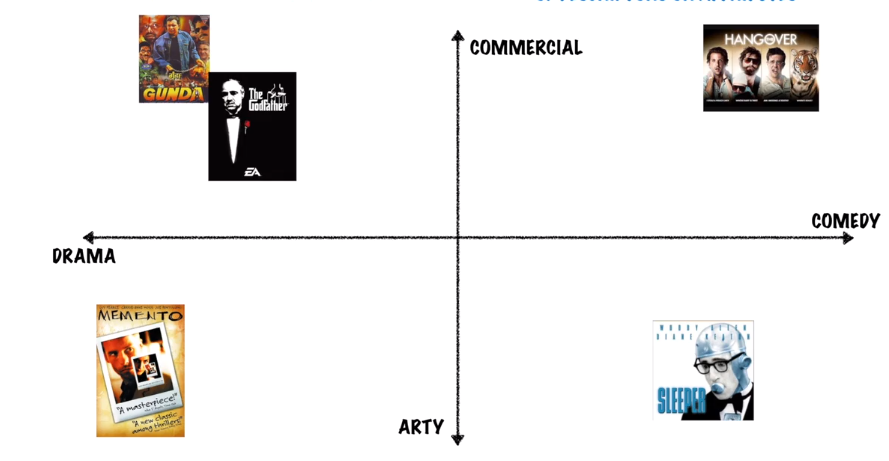
\includegraphics[scale=0.6]{content-based}
\caption{Movies are mapped on a scale that define how much dramatic/comedy and commercial/artistic they are.}
\end{figure}

Users and items needs to be prepared before they can be used in a content-based filtering algorithm. Items have to be represented as vectors with attributes as dimensions that can be binary or real numbers in a range between 0 and 1. Each user is represented by his history of liked items using the same items attributes. As example, in a recommender system about movies where user and item are represented in a drama-comedy/arty-commercial space, if a user has liked 10 movies, 7 of which commercial and 3 drama, his vector representation would be something like (-0.9, 0.7) where X-dimension is the drama-comedy value and Y-dimension the arty-commercial attribute placing the user in the graph near the drama-commercial movies. Once all its represented with vectors and placed in the graph, recommendations are possible thanks to the nearness of user points to the items points. The main problem with this type of algorithms is the difficulty to find classified data: each item has to be classified with its attributes and this process it is not always straightforward. First of all, there is the problem to choose the attributes of the items and then to find how to measure them, as example, given a movie, it is hard to know if it is drama or comedy without a manual classification. So, data needs to be manually classified and this can be very tedious. This difficulty makes content-based filtering approach less used compared to other algorithms of recommendation system.
One successful application of content-based filtering is the Music Genome Project by Pandora Radio. The idea is to associate descriptors to each song. Each song is described by a vector of 450 "genes" manually generated by professional musical analysts. Genes are songs properties like the tempo, the pitch, the frequency and more. Once every song has its own attributes, users can start to like songs and the algorithm can do his recommendations. This is the concept behind Pandora Radio.

\subsubsection{Collaborative filtering}

Collaborative filtering algorithms takes inspiration from what happens to the real life when we are searching for recommendations: we ask a friend. This relies upon the idea that if two people have same opinions about a group of items, then it is likely that they have the same opinion on other items too. Every algorithm that is based on the user behavior (history, reviews, similarity) belongs to the branch of collaborative filtering algorithms. Unlike content-based, collaborative filtering does not require items to be classified, instead, this algorithm can be used even with absolute no knowledge about the items that are going to be recommended.
This types of algorithms tries to predict the reviews of a user to a product he has not reviewed yet. Review is a generic term and can be referred to a positive-only feedback, where user has liked/not liked the item, an explicit review, where the user assigns a number (typically on the Likert scale from 1 to 5)  to the item, or an implicit review made of all the metadata about a user, like the numbers of clicks, the time spent viewing a product, his temporary shopping cart, his researches or his history of purchased products or digital goods consumed. 
Of all the collaborative-filtering algorithms available, two in particular has gained popularity in the community: the Nearest Neighbor algorithm and the Latent Factor algorithm.
The Nearest Neighbor algorithm finds user that are similar to other users, using a metric for the similarity and a metric for the distance between users.
The Latent Factor algorithm tries to find common factors between users from the reviews they already gave to items.

\subsubsection{Hybrid recommender system}

As the name suggest, hybrid recommender systems combines collaborative filtering and content-based filtering to obtain the best of both worlds and to overcome some of the common problems in recommender systems such as cold start, gray sheeps and the sparsity problem (discussed in the following section). Several studies  \citep{hybrid_rs} empirically compare the performance of the hybrid with the pure collaborative and content-based methods and demonstrate that the hybrid methods can provide more accurate recommendations than pure approaches. There are several ways to implement an hybrid approach: one can be making the content-based and collaborative-filtering prediction separately and then combining them; predictions are based on a weighted average of the content-based recommendation and the collaborative recommendation. The rank of each item being recommended could be a measure for the weight. In this way the highest recommendation receives the highest weights. Another technique is to add content-based capability to a collaborative-based approach or viceversa; since collaborative filtering looks for the correlation between user ratings to make predictions, finding such correlation can be unfeasible for users with few ratings. Adding content information to the recommender system can help to correlate users. For example, if one user liked the movie “Rocky” and another liked the movie “Rocky II” they would not necessarily be matched together. A hybrid approach deals with these issues by incorporating both the information used by content-based filtering and by collaborative filtering.
\\
Netflix, a popular streaming media platform, uses an hybrid recommender system. The website makes recommendations by comparing the watching and searching habits of similar users (i.e., collaborative filtering) as well as by offering movies that share characteristics with films that a user has rated highly (content-based filtering).


\subsection{Current state and limitations}

Latest studies   \citep{RS-ML1}  \citep{RS-ML2} have shown the utility of machine learning techiniques in the area of recommendation systems and information retrieval. The general opinion is that of significant improvements over the conventional models. Although this trend has covered all the three major variants of recommender systems algorithms, collaborative filtering, content based and hybrid systems, it can be clearly seen from the number of publications made, that the majority have leveraged deep learning to enhance collaborative filtering capabilities. As example, deep learning can be used to help classify data for content-based algorithms or to replace matrix factorization with deep neural networks for collaborative filtering. 
Most of the deep learning development has been biased towards entertainment industry such as in movie and music recommendation. This can be largely attributed to the availability of rich datasets for validation. 
Unfortunately, recommender systems have a set of problems and limitations   \citep{RS-stateofart} that has to be taken into account: \textit{cold start, synonimy, gray sheep, data sparsity} and \textit{shilling attacks} to name some. 

\subsubsection{Cold start} The cold start problem addresses the case of new items or new users in the system: since they have no ratings history, find good recommendation can be tricky for them. One of the solutions is to use an hybrid system called content-boosted collaborative filtering that combines known attributes of items with demographic data  of users to improve collaborative filtering recommendations.

\subsubsection{Synonimy} Synonimy occurs when the algorithm has to deal with items that are practically the same but differs from a single or few attributes, like two different editions of the same book; latent factor collaborative filtering works well with these cases.

\subsubsection{Shilling attacks} Shilling attacks is the name given to the problem of dealing with users that wants to fool the recommender system. As example, think at a restaurant owner that gives fake negative reviews to other restaurant while using fake accounts to give positive reviews to his restaurant. In that cases, precautions is the best weapon.

\subsubsection{Data sparsity} Data sparsity occurs when a lot a of users have reviewed only a few items: this makes the user-item matrix very sparse, resulting in hardness to compute the prediction and unsatisfied results. The solution is to use dimensionality reduction to remove less important dimensions in vectors to reduce sparsity.

\subsubsection{Gray sheeps} Gray sheeps are users with non-consistent opinions. The hypothesis on which collaborative filtering algorithms are based that is, if two users likes the same item and one of them likes another item, that item may interest the other user too, it's false with gray sheeps. Content-boosted collaborative filtering can help dealing with this problem.

\section{Personalization}

\subsection{Introduction}

With the enormous amount of available data on the web today, there is the need to filter out what really interests users. Data filtering can improve user engagement in entertainment applications, can enhances revenues of online shopping portal (think about what Amazon does with "Customers who bought this item also bought") and can help search engines to give better query results. Recommender systems were built to overcome the problem of data filtering but they only relies upon items attributes and users history, with little "real-life" relation to the user. There are strong desires to provide online users more dedicated and personalized services that fits into individual's need, usually strongly depending on the inner personality of the user. 
Canada Peer Counseling Center   \citep{chen} considers that for most people they have investigated, recommendations from companion volunteers with same views as being the most effective. It means people with same personality tend to attract each other. As a result, analysis of different personality features can be the basis for building characterized service. For example, an extrovert user may have a higher level of online activity which is more likely to use recommendation system to make new friends with strangers   \citep{moore}.

\subsection{Background}

Personality is defined as the set of habitual behaviors, cognitions and emotional patterns that evolve from biological and environmental factors   \citep{gerald}. The study of the psychology in personality, attempts to explain people's differences in behavior. Many approaches have been taken to study personality, including biological, cognitive, learning and trait based theories, as well as humanistic approaches. Following, there will be a description of two approaches used for scientific applications thanks to their numerical nature: the Five Factor Model and the Myers Briggs Type Indicator.

\subsubsection{Five Factor Model}

The Five Factor Model (FFM), also known as the Big Five Model (Big5), is a model based on common language descriptors of personality. The model mainly relies upon two theories: the lexical hypothesis according to which it is possible to derive a comprehensive taxonomy of human personality traits by sampling language, and a statistical approach which identifies the characterizing dimensions of individual differences through a factorial statistical analysis.
Studies on the personality lexicon   \citep{lexicalapproach} started in 1884 by an English psychologist, Sir Francis Galton, who extracted 4504 adjectives from the dictionary which he believed were descriptive of observable human personality traits   \citep{galton}. This number was reduced by successive studies, first to 171 by eliminating synonyms, then to only 20 and finally to five broad factors which were labeled: \textit {Agreeableness, Conscientiousness, Extraversion, Neuroticism} and \textit{Openness}, also known as OCEAN:

\begin{itemize}

    \item \textit{Agreeableness} refers to being helpful, cooperative, and sympathetic towards others. Low Agreeableness is related to being suspicious, challenging and antagonistic towards other people.
    
    \item \textit{Conscientiousness} is determined by being disciplined, organized, and achievement-oriented. Low Conscientiousness individuals tend to be more tolerant and less bound by rules and plans.
    
    \item \textit{Extraversion} is displayed through a higher degree of sociability, assertiveness, and talkativeness. People low in extraversion are reserved and solitary.
    
    \item \textit{Neuroticism} refers to degree of emotional stability, impulse control, and anxiety. Those who have a low score in Neuroticism are more calm and stable.
    
    \item \textit{Openness} is reflected in a strong intellectual curiosity and a preference for novelty and variety. People low in Openness tend to be more conservative and close-minded.
    
\end{itemize} 

An example of personality questionnaire is The Revised NEO Personality Inventory from Costa and McCrae . It consists of 240 items on a five-point likert scale, and can accurately 105 measure the five personality traits plus six underlying facets for each of them

In 1985, psychologists McCrae and Costa developed a personality inventory called \textit{The Revised NEO Personality Inventory} (NEO PI-R,   \citep{NEOPI-R}) that makes the Big Five personality traits measurable. The inventory consists of 60 questions in his shorter version and the traits are expressed as dimensions of a vector in a scale between 0 and 1. 

\subsubsection{Myers Briggs Type Indicator}

In 1920, two psychologists, Katharine Cook Briggs and her daughter Isabel Briggs Myers, have developed a convenient way to describe the order of Jungian preferences of a person. Their work is based on the Jungian theory of personality described in his book \textit{Psychological types}, in which he describes the different characteristics of attitudes and behaviours. Jung mainly splits individuals in two categories, Introverts and Extroverts which represents the guidelines both in the objective and subjective world. Then, he postulated that individuals relate to the world through two sets of opposed functions, rational functions of thinking and feeling and irrational functions of sensation and intuition. Jung work is descriptive and general, which from one side, leaves personal interpretation opened but on the other, makes hard to outline personality attitudes precisely. Myers and Briggs, facing these difficulties, have extracted the more easily distinguishable personality traits from Jung work on which they added a personal contribute based on a more traditional psychometric procedures. The result of their studies is a set of intrinsically consistent indices that measure the differences in behaviour of individuals. The set is made by four indexes, Extraversion-Introversion, Sensing-Intuition, Thinking-Feeling and Judgment-Perceiving. The last is their contribution to Jung's work. Each index is dichotomized, with a center-fixed zero point and represented by two letters which indicate the ends. They indicates how people:

\begin{itemize}
    \item Focus attention and energy (Extraversion-Introversion)
    \item Extract informations from the surrounding world (Sensation-iNtuition)
    \item Take decisions (Thinking-Feeling)
    \item Relate to the external world (Judging-Perceiving)
\end{itemize}

The combinations of these four indexes outline 16 possible psychological types. For instance, ESTJ means a profile made the following attributes: extraversion (E), sensing (S), thinking (T), judgment (J) while INFP means introversion (I), intuition (N), feeling (F), perception (P). 

\subsection{Personality and computer science}

Knowing the user personality can help to make better recommendations considering that people with same personality tends to attract each other. Since collaborative filtering recommender systems mainly relies on users online history, there is the need to find a way to predict personality from their behaviors. In psychological researches, most traditional personality analyzing experiments are based on self-reported inventory. Self-Report Measures are any methods of data collection that rely on the participant to report his or her own behaviors, thoughts, or feelings. The advantage of this method is that the researcher can obtain information that is not easily observable, but the disadvantage is that participants' report may not be accurate or reliable. For example, if we asked students to report how many hours per week they used Facebook, students may under-report the time due to embarrassment or not realizing how much time they spend on the site. However, independent observation of Facebook use would be difficult and costly to implement.
Other data collection methods such as observable information profile cost a lot of manual resources and are not desirable for large scale of dataset collection. At the same time, most personality researches can only build the covariation relation between behavior and personality instead of a quantitative personality prediction.
To solve these problems, several studies proposed an approach to predict personality, by means of Big-Five or MBTI, from user's social networks behaviors. Bai et al. (2012), in their paper \textit{Big-Five Personality Prediction Based on User Behaviors at Social Network Sites}, have built a model to predict personality of RenRen users, a Chinese social network. University of Cambridge Psychometrics Centre developed a web application called Apply Magic Sauce, based on artificial intelligence whose models are based on over 6 million social media profiles and matching scores on psychometric tests; This gives the ability to predict user's personality from their digital footprint.    


\chapter{Approach}

\section{Introduction}

This chapter is dedicated to present the architectural work required before Chatbot implementation, first from an high-level perspective, showing how components are bound together to work and communicate, and then exploring every single component, what they are, what they do and why I decided to choose them. 

\section{High-level Architecture}

 To explore the various aspects which I had to take into consideration while architecting the chatbot application, is useful to start from the words of the thesis title.
 First word, \textit{Multi-channel}, means that the chatbot has to be
 accessible from a variety of platforms that offers the chatbot service and the users has to be recognized between all of them. For the first functionality, I had two main alternatives: write the code for every single platform or use a middleware. Fortunately, thanks to the growing popularity of chatbots, there are a lot of good middlewares called \textit{Chatbot Builders} that can handle both conversational logic and multi-channel aspect of chatbots. To allow users authentication, I decided to use a login system built in a website that directly communicates with the webserver and can be easily accessed from a link provided as the first message on all the platforms. The \textit{Conversational Agent} aspect is covered in part by the chatbot builder as for routing user requests to correct responses, and in part by an Apache webserver that builds the responses, hosted on a machine property of Istituto Superiore Mario Boella research centre. As for \textit{Personalized Music Recommendations}, first I have to explain what \textit{Personalized} means in this application context. The chatbot recommends music artists to users and those are chosen on a preference inferred by the user personality. To compute users' personalities, I had to choose between subjecting users to a psychological assessment or use a affective computing service to predict personality. Given the fact that a psychological assessment requires at least 10 to 15 minutes to be completed, affective computive appears a more viable way for an entertainment product like a music recommender chatbot.  The last aspect which I had to take into consideration is \textit{Music Recommendations}. Here the obvious choice is to use a modern Recommender System, that are the state-of-the-art approach to give recommendations today  \citep{Singhal}. As for data, I decided to use a SQL database mainly for the ecosystem: SQL has 40 years of existence and this means an enormous amount of already solved problems and informations are available today on the web. Another reason is that SQL also support JSON object storage. 
To recap, the chatbot application, named \textit{Beat in a Bot} is made of different components: a chatbot builder to handle the conversational flow and the multi-channel aspect, a website to provide shared authentication between the different platforms and to show the results of the personality prediction, a recommender system to provides personalized recommendations, a SQL database to store users and artists data, a web server to handle the dialog fulfillments, manage the database operations, execute the recommender algorithm, make requests to the affective computing service and Facebook Graph and manage the authentication requests from the website.

\begin{figure}[h]
\centering
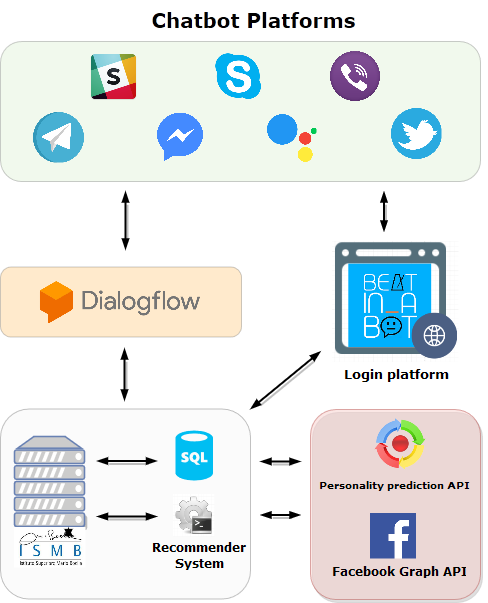
\includegraphics[scale=0.39]{architecture.png}
\caption{The system architecture}
\end{figure}

\section{Building components}

\subsection{Dialogflow}
Dialogflow, formerly known as \textit{Api.ai}, is a developer of human-computer interaction technologies based on natural language conversations. The company, is backed by Google and runs on Google infrastructure, which means it can scale to millions of users. Once designed, the conversational app can be easily deployed to a variety of platforms with a one-click integration. Dialogflow supports more than 14 languages allowing developers around the world to make their conversational agents in their preferred language. 

\subsubsection{Fundamentals}

Dialogflow basic concepts are: \textit{Intents, Entities, Events, Contexts} and \textit{Actions and Parameters}. The process a Dialogflow agent follows, is similar to someone answering a question. In order to start a conversation with an agent, the user needs to invoke it. A user does this by asking to speak with the agent in a manner specified by the agent developer that can be an \textit{event} or a keyword that triggers an \textit{intent}. In Dialogflow, an intent houses elements and logic to parse information from the user and answer to their requests. For the agent to understand the question, it needs examples of how the same question can be asked in different ways. Developers add these permutations to the User Says section of the intent. The more variations added to the intent, the better the agent will comprehend the user. Dialogflow uses machine learning to understand what users are saying, more specifically, it uses natural language understanding techniques.
\\
\noindent
The Dialogflow agent needs to know what information is useful for answering the user's request. These pieces of data are called entities. Entities like time, date, and numbers are covered by system entities. Other entities, like weather conditions or seasonal clothing, need to be defined by the developer so they can be recognized as an important part of the question.
\\
\noindent
Dialogflow agent can respond to the user questions in two ways: with hardcoded text responses provided by the developer in the "Text response" section or by providing a \textit{webhook} to an external webservice, which subsequently fetches the data needed, determines how it would like to respond, and sends it back to Dialogflow. What makes Dialogflow a real conversational agent is the concept of \textit{Contexts}. Context can be used to remember something from one intent to another. For instance, if the first intent was triggered by "\textit{What's the weather supposed to be like in San Francisco tomorrow?}", information can be saved in the form of \textit{parameters}, which can be the \textit{city} we would like to know the weather about. The next intent can be \textit{"How about the day after that?"} and because the agent knows previous information thanks to the context parameters, it can replies with the San Francisco forecast for the day after. Contexts are also used to repair a conversation that has been broken by a user or a system error, as well as branch conversations to different intents, depending on the user's response. 

\begin{figure}[ht]
\centering
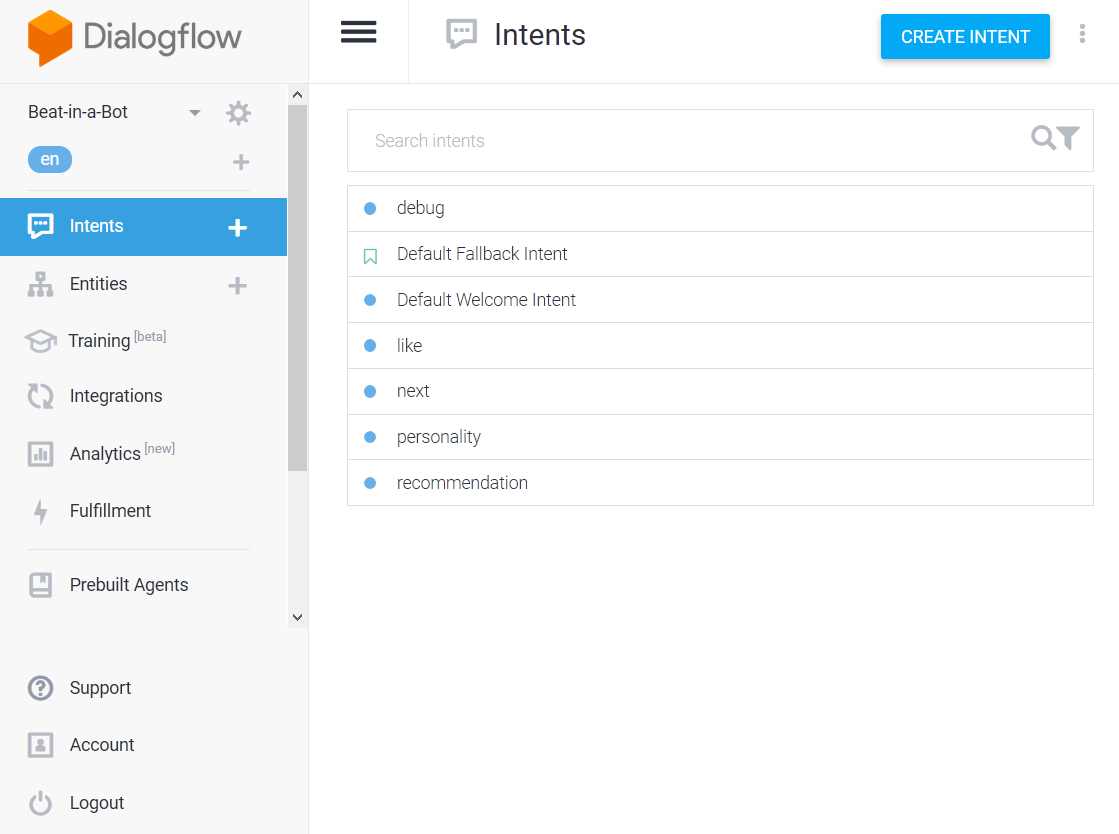
\includegraphics[scale=0.47]{dialogflow_console.png}
\caption{The Dialogflow console.}
\end{figure}

\subsubsection{Multi-channel}

Dialogflow provides a one-click integration to deploy the conversational agent on many different messaging platforms. The process works as follows: when on the \textit{Integrations} section of the Dialogflow console, the developer select the platform he wants to deploy on. Once selected, a window showing the instructions to make the integration appear; after all is set in the correct way, the conversational agent start to work on the platform. As example, if the user wants to deploy the agent on Telegram, he needs to start a conversation with BotFather bot as stated in the Telegram documentation. Developer needs an access token from BotFather that to be copied and pasted into the Dialogflow window. When done, the integration can be completed by pressing the button "start".

\begin{figure}[ht]
\centering
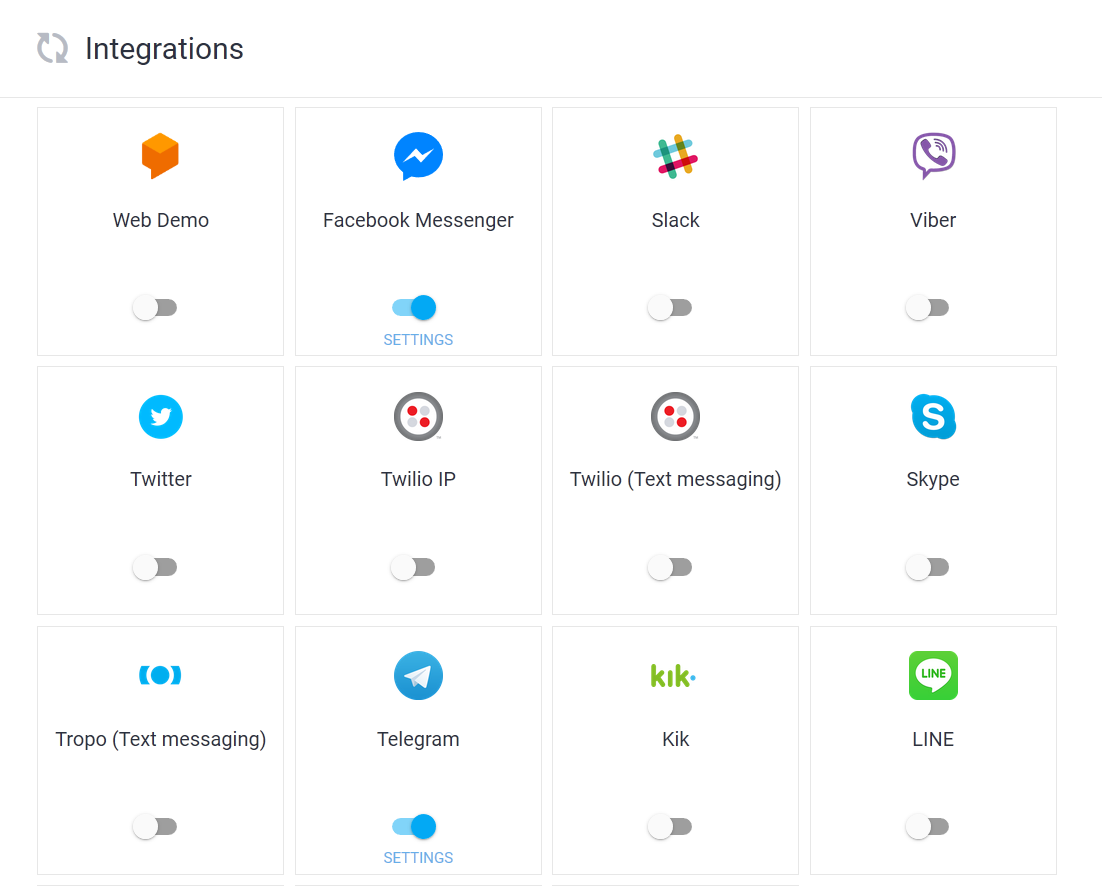
\includegraphics[scale=0.53]{dialogflow_integrations.png}
\caption{Integrations section of Dialogflow console.}
\end{figure}

\subsubsection{Rationale for the choice}
I decided to use Dialogflow rather than other platforms because at the same it is simple and powerful, it is reliable thanks to the Google backend and has the possibility to easily deploy the conversational agent on many different platforms. This eliminates the need to re-write the code for each messaging platform making the developer work easier.


\subsection{MyMediaLite}

MyMediaLite is a recommender system library for the Common Language Runtime (CLR, often called .NET). It is a free and open source software and was developed by Zeno Gantner, Steffen Rendle, Lucas Drumond, and Christoph Freudenthaler at University of Hildesheim.
MyMediaLite can be used as an executable file or can be imported as a library in personal project. It has many recommendation methods that can use collaborative and attribute/content data; since is written in C{\#} for the .NET platform, it can run on every architecture supported by Mono as Linux, Windows and Mac OS X. The core library of MyMediaLite, as the name says, is leaner and simpler and carries less overhead; it has a size around 150KB and does not require a database to work. It takes as input text files that have to be in a particular format.
MyMediaLite includes evaluation routines for rating prediction and item prediction; it can measure MAE, RMSE, CBD, AUC, prec@N, MAP, and NDCG. Other additional features are:

\begin{itemize}
    \item Serialization: save and reload recommender models
    \item Real-time incremental updates for many recommenders
	\item Attribute-based diversification of recommendation lists
\end{itemize}
 
MyMediaLite addresses the two most common scenarios in collaborative filtering:
\begin{itemize}
    \item rating prediction (e.g. on a scale of 1 to 5 stars)
    \item item prediction from positive-only feedback (e.g. from clicks, likes, or purchase actions).
\end{itemize}

\subsubsection{Most Popular and ItemKNN algorithms}
%%% da fare %%%%


\subsubsection{The Cold Start problem}
It is known that a recommender systems to works properly needs a user history on which building recommendations. Suppose the case of a Collaborative Filtering algorithm; the system is based on similarity between users but how to deal with new users? New users are a problem for recommender systems because there isn't enough data to define their profile so that similarity with other users can be measured. This problem takes the name of \textit{Cold-start} problem because, as a car with a cold engine has troubles to start up, a recommender system algorithm doesn't do his best when started with few data.
There are several solutions to the problem:

\begin{itemize}
	\item \textit{Popularity based strategy}: Global trends and popularity of products can be used, as well as what's popular it the area of the user or in a particular hour of the day.
	\item \textit{Contextual information}: Several information can be exploited from the user profile like his position, the website he come from, his operating system and his browser.
	\item \textit{Use of a personality model}: Using a personality model like the Five Factor Model or the MBTI, a initial profile of the user can be created on his personality.
	\item \textit{Community information}: Data can be extracted from a community the user belongs to. As instance, information about a user gathered from a recommender system that works on Amazon can be user for another that operates on eBay. Another example can be, assuming that two users are friends and they like the same books, probably the will like same movies too.
	\item \textit{Decision tree}: a decision tree classification model can be used. The tree is build on the properties of the users that already are in the dataset.
\end{itemize}

The approach I take to solve the problem is the use of a personality model. Since my application requires by design the prediction of the user personality, I can use this information to build some initial recommendations. The idea is to start with the most popular artists of the musical genres bounded with the personality profiles. As example, a personality of the type INTP is linked with the vector of genres in descending order of preference: Rock, Alternative, Classica, Electro, Pop, Jazz, Ambient, Punk. The server runs MyMediaLite recommender system with the MostPopular algorithm on the LastFM dataset, returning the list of the most popular artists. The recommendations given is the set of the first artists of each genre of the vector found by looping on the Most Popular list so that the result is: most popular rock artist, most popular alternative artist and so on. Once I have enough preferences, those can be grouped by the different personalities of the users. This allows to give better recommendations truly based on personality profiles.

\subsubsection{Rationale for the choice}
I decided to use MyMediaLite as a recommender system because it is a ready-to-use package and this allowed me to easily integrate it in my solution. MyMediaLite is also the most popular library in the recommender systems community. Another reason for the choice is a personal preference for open source software and to conclude, MyMediaLite it is also used by researchers of Istituto Superiore Mario Boella, the research center where my thesis was born; this gave me the added value of having a live community support to the usage of the application.

\subsection{Apply Magic Sauce}

Apply Magic Sauce is an application developed by The Psychometrics Centre, a Strategic Research Network of the University of Cambridge, centre of excellence in psychological, occupational, clinical and educational assessment  \citep{applymagicsauce}.  It is released with the \textit {Software as a service (SaaS)} paradigm which includes a web application and a RESTful Web service. Apply Magic Sauce is powered by an artificial intelligence algorithm and its model is trained on over 6 million social media profiles and matching scores on psychometric tests. It takes as input a \textit{digital footprint} that can be a list of Facebook likeIDs, Facebook statuses, tweets, user browsing data, open text and other and gives as output an Individual profile containing psychographics and demographics. 

\begin{figure}[ht]
\centering
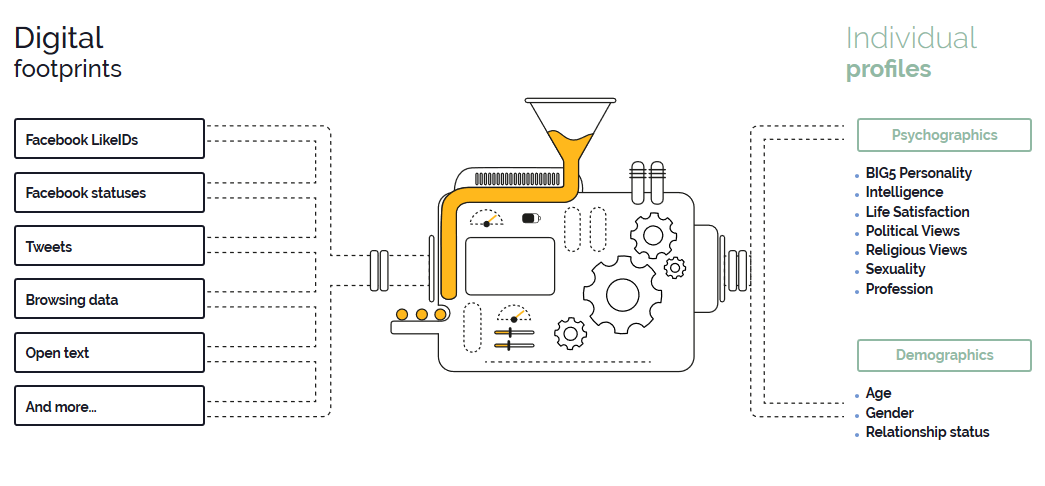
\includegraphics[scale=0.455]{ams.png}
\caption{The Apply Magic Sauce Trait Prediction Engine from \url{https://applymagicsauce.com/about_us.html}}
\end{figure}

\noindent
Apply Magic Sauce goal is to solve the problem that Machine-learning algorithms can be difficult to interpret, let alone implement in a product. These algorithms are at risk of perpetuating historical prejudice, being overly domain-specific or prescribing norms that can feel impersonal. Apply Magic Sauce API enables conversation between businesses and consumers about how predictive technologies ought to be used. This could help algorithms explain themselves and learn from their mistakes, just like humans. Once predicted, psychological data points can be added to any sample data our devices records, making them a valuable resource that can be used to tailor online experience on the different personalities.

\subsubsection{Rationale for the choice}
%parla anche di Traitify%

To predict user's personality, I had to choose between subjecting users to a psychological test or use an automated system like Apply Magic Sauce. The first choice has the advantage of not having any requirement but, to be reliable, the test have to last at least 10 minutes due to the number of questions needed. The second choice is only feasible if the user has a Facebook account with a sufficient number of likes for the service to work, but it is fast and enough reliable (it depends on the "quality" of user likes). I decided to choose Apply Magic Sauce for the speed of the process, taking into account the fact that users tends to uninstall apps if they require a tedious process to start up  \citep{clevertap}. 

\subsection{Facebook Graph API}

On April 21, 2010, during the F8 Live event, Facebook presented a series of news about the way to develop applications for the social network. The most important were the adoption of the OAuth 2.0 authentication standard, three new SDK, for Javascript, Python and PHP and a new API called \textit{Graph API}. Graph API is described as "the primary way for apps to read and write to the Facebook social graph  \citep{graphapi}". Technically speaking is a low-level HTTP-based API that developers can use to programmatically query data, post new stories, manage ads, upload photos, and perform a variety of other tasks that an app might implement. Facebook Graph API is based on the concept of \textit{graphs}. Graphs are mathematical structures, composed by elements called \textit{nodes} linked together by \textit{edges}. Those structures extend their field of application way beyond mathematics, reaching computer science, sociology and so Facebook. The idea behind the Graph API is to consider elements like users, pages, photo, video, comments and others as nodes of the graph (called \textit{objects} in Facebook semantics) and connections between them as \textit{edges}. There also are \textit{fields} that represents information about objects. For instance, \textit{friend} connections links together \textit{user} nodes and \textit{likes} connections links a user to the pages he likes. The Graph API is HTTP based so it can be used with any language that has an HTTP library. Each node has an unique ID which is used to access it via the Graph API. The following example shows how to make a request to the graph:

\begin{verbatim}
    GET graph.facebook.com
        /{node-id}
\end{verbatim}

\noindent
Responses are always formatted as JSON objects. The response of a request made with Politecnico di Torino page-id, has the following format:

\begin{verbatim}
{
  "about": "Pagina ufficiale del PoliTo su Facebook",
  "name": "Politecnico di Torino",
  "fan_count": 60254,
  "picture": {
    "data": {
      "height": 50,
      "is_silhouette": false,
      "url": "https://scontent.xx.fbcdn.net/v/p50x50/polito.jpg
      "width": 50
    }
  },
  "id": "17570259916"
}
\end{verbatim}

To request for edges instead, the syntax is:

\begin{verbatim}
    GET graph.facebook.com
        /{node-id}/{edge-name}
\end{verbatim}

\noindent
It is also possible to push by making HTTP POST requests and to delete using HTTP DELETE requests to the same endpoints.

\subsubsection{Rationale for the choice}
The choice of using this tools is linked to the usage of Apply Magic Sauce web service. To predict users personality profile, the list of all their likes to Facebook pages is needed. The only way to 
programmatically retrieve such lists is the Facebook Graph API.

\subsection{Website and login platform}

The supporting website is a web page that allow user to authenticate with the OAuth 2.0 Facebook Login method and to ask the web server continue with the operation of predict user's personality profile. It also gives additional information such as a brief description of the user's personality (taken from the official website of the Myers-Briggs Foundation   \citep{MBfoundation}), the Facebook pages that determines the four dimensions of MBTI and a list of music artists with same user's personality. The first time a user chat with the bot (on each platform), he is presented with the URL of the website and instructions on how to proceed. The website is structured as a to-do list with two entries: first it is asked to log in with Facebook Login and then to press a "Start" button. The first action allows to retrieve the user's name, his facebook ID and Access Token that can be used to extract his likes to Facebook pages, while the second action sends those data, together with the user's Dialogflow sessionId, to the web server. If all the operations runs successfully, a "Back to the bot" button appears, together with the other information gathered.

\begin{figure}[ht]
\centering
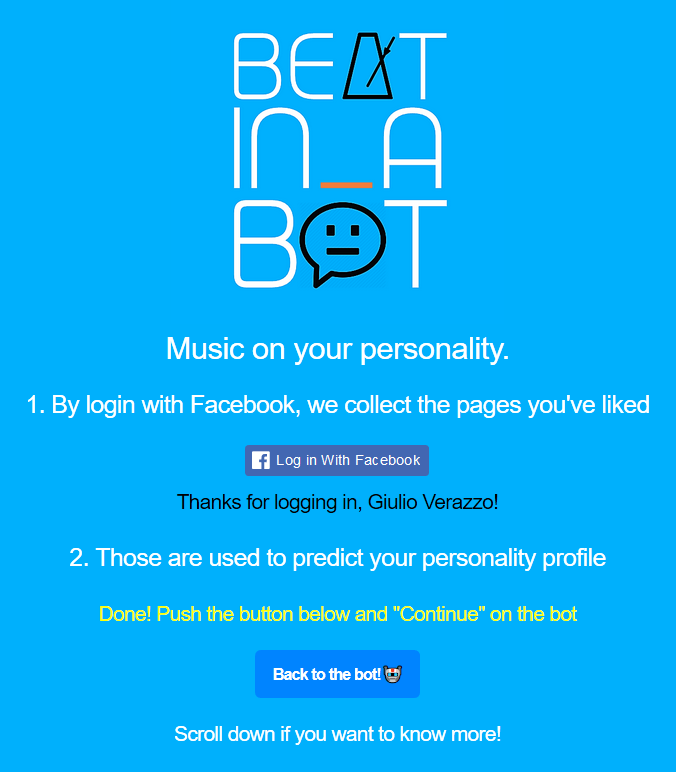
\includegraphics[scale=0.65]{website1.png}
\caption{The login screen.}
\end{figure}


\subsubsection{Rationale for the choice}
%scrivi perché l'hai fatto
The choice of developing a supporting website for the chatbot application is essentially bound to two previous architectural choices: first one, the Multi-channel support, automatically implies to have a flexible authentication method that can be used independently of the messaging platform chosen to interact with the bot. This is required because every single platform has its own login system and it's up to developers to manage them. The other, is a direct consequence of the choice to use Apply Magic Sauce web service, which requires data from the user's Facebook profile to make the personality prediction. Since Apply Magic Sauce also accept user's Tweets as input, a possible extension for the website could be to allow users authenticate with Twitter also. This soften the actual pre-requisites of the application, allowing more people to use the service. As for the website hosting, I chose \textit{GitHub Pages}, an hosting service offered by GitHub. It is free and it allows developers to host directly from GitHub repositories, having all the benefits of the git versioning plaform like commit, push and pull to manage the website. 
\subsubsection{How it works}
%scrivi come l'hai fatto non dimenticare di menzionare dove è hostato e perché e che hai usato HTML5UP come template e perché 
The supporting website is developed using modern technologies for web developing like HTML5, CSS3, JavaScript and the JQuery library; rationale of choice is that these technologies are largely used by the web developers community and this represent added value in terms of technical support. The site is built upon a template by HTML5 UP  \citep{html5up} which provides free, customizable and fully responsive templates for the web. This allows me to have a web site that adapts easily on the different form factors of the screens of smartphones and tablets as well as desktop and notebooks. As for the hosting, I decided to use GitHub Pages   \citep{githubpages}, a service that gives the opportunity to host directly from the GitHub repository for free. From what regards developing details, I used Facebook JavaScript SDK to implement Facebook Login authentication system and the JQuery library to make an asynchronous GET request to the server. When user starts a new chat session, a link having the following URL is provided:

\begin{verbatim}
https://giulioverazzo.github.io/beatinabot_website
/?sessionId={sessionId}
\end{verbatim}

\noindent
The sessionId parameter is extracted from the server by Dialogflow and is needed to authenticate the user and to link the chat session to the website. This allows the server to know which user is making requests from the website. When the user clicks on "log in with Facebook" button, a window appears showing the permissions required for the app to work. Those are: \textit{email, public\_profile, user\_friends} and \textit{user\_likes}. Once accepted, the user is logged in and his ID, name and access token are sent from Facebook to the website. The final step occurs when he clicks on "Start" button; this triggers an GET request using AJAX to the server URL:

\begin{verbatim}
http://datascience.ismb.it/beatinabot/hello?userid={userid}
&accessToken={accessToken}
&name={user_name}
&sessionId={sessionId}
\end{verbatim}

\noindent
When the server receive the request, it checks if the user is already known by the system and it does it by checking if the Facebook userID is in the database. If so, it replies without requesting the profile prediction to Apply Magic Sauce, otherwise it does. In case of error, it replies with a proper error message. 

\subsection{Web server}

A web server is a software application that runs on a computer called \textit{server} and is in charge of handling requests from a \textit{client}, typically a web browser. It uses the HTTP (\textit{HyperText Transfer Protocol}) protocol, the basic network protocol on the World Wide Web. Main purpose of a web server is to process and deliver web pages to clients but they can also run operations written in a server-side scripting language as ASP, PHP, Python or Node.js. This allows to deliver dynamic web pages and to retrieve and modify information from databases.
In my application context, the web server has four main purposes:
\begin{itemize}
    \item Acts as webhook for Dialogflow \textit{Fulfillments} feature
    \item Communicates with Facebook Graph API
    \item Communicates with Apply Magic Sauce API
    \item It manages the database operations
\end{itemize}

\subsubsection{Webhook}
Webhooks are defined as "user-defined HTTP callbacks"  \citep{fitz} i.e. when an event occurs such as pushing code to a repository or commenting a post on a blog, the source site makes an HTTP request to the URL configured as a webhook; tipically events on one site invokes behaviour on another and the action taken may be anything. The main reason behind webhooks is to augment or alter the behaviour of a webpage or a web application. 
\\
Dialogflow, the chatbot builder chosen as a middleware for this project, allows developers to define a webhook URL where requests will be made when an Intent is triggered. When this event happens, if the Intent requires an external fulfillment, Dialogflow sends to the webhook, a properly formatted JSON object that includes information about the triggered Intent, the original request, the conversation context and other metadata about the session and the user. When the webserver receives the request, it replies accordingly to the data received.

\subsubsection{Facebook Graph API}
The first time a user speaks to the chatbot, a link to a website is presented to him; on the website, the user has to first authenticate with Facebook Login and then, he have to press a button that starts the computation of his personality profile. An app which implements Facebook Login as the website, is able to obtain an access token which provides temporary, secure access to Facebook APIs. An access token is an opaque string that identifies a user, app, or Page and can be used by the app to make graph API calls. Basically, with an access token, information on a node (a user, a page or other) can be retrieved from Facebook. So, what the website does, is to first obtain the user access token and then send it to the webserver to make him able to retrieve the list of user's likes to Facebook pages.

\subsubsection{Apply Magic Sauce API}
Once obtained, the list of user's likes to Facebook pages can be sent to the affective computing service \textit{Apply Magic Sauce} that expose a so-called "Prediction API" where information about user psychological traits can be retrieved from his "digital footprints". In this case, the webserver sends the list of likes as input to the APIs (the digital footprints) and the BIG5 traits and Myers-Briggs Type Indicator are returned as output (the psychological traits); moreover, with each BIG5 trait, a list of the likes used in positive or in negative i.e. the ones that determine or exclude the trait, is returned. Those data are sent back to the website as a result of the computation started when the "Start" button in pressed. 

\subsubsection{Database operations}
The webserver is in charge of establishing a connection with the SQL database and doing all the queries needed for the application. It has to fill and keep updated the table of users with all their ids and metadata, extract the recommended artists information from their ids retrieved from the recommender system, save and keep track of the recommendations for each user, it stores the JSON objects gained from \textit{Apply Magic Sauce} to show users how the pages they liked on Facebook relates with the four dimensions of their personality, it checks if a user is already signed in the application, it stores the likes to recommended artists given by users on the chat and finally it manage all the "next" requests. 

\subsubsection{Rationale for the choice}
I have chosen to add and develop a webserver in the application architecture to implement and expand the functionalities offered by the chatbot. The webserver is vital for the majority of the operations (described in the sections above) and without it, only a small amount of possibilities are available, i.e. the ones offered by the chatbot builder alone. I chose Python as the main programming language for the server, mainly for the large variety of packages available, its compatibility with all the other software used and the support of the huge community on the web. Python is also a preferred language between researchers at Istituto Superiore Mario Boella, where I worked during the making of this thesis project. As for the hosting, the python script runs under Flask, a micro web framework to easily implement a web server i python with very few lines of code. The URL mapping is managed instead by Apache, the most commonly used HTTP server over the net.

\subsection{Database}
A fundamental piece of the developed architecture (and every other web application) is the database. A database is a collection of information that is organized so that it can be easily accessed, managed and updated. In a relational database, where information is modeled as relations between sets of objects, data is organized into rows, columns and tables, and it is indexed to make it easier to find relevant information. Data gets updated, expanded and deleted as new information is added. Databases process workloads to create and update themselves, querying the data they contain and running applications against it. 
\\
There are several types of database available today and, depending on the nature of the application and of course the preferences of the developer, one can be preferred over another to better fit the project needs.
The database chosen for this chatbot application is a relational database called \textit{MySQL}. MySQL is a Relational Database Management System (DBMS) made of a command line client and a server; both are available on Unix and Windows systems and it is release as an open source software. It supports a large variety of programming languages live Java, Mono, .NET, PHP, Python and many others. In the context of my application, the database contains data about artists, users and their personal recommendations.

\subsubsection{Dataset used}

%aggiungi un esempio di dataset e alcune statistiche (Come nel paper di Giulio)
 
To make recommendations possible with no history about users' preferences, the database has been initialized with data from \textit{hetrec2011-lastfm-2k}, a dataset built by Ignacio Fern{\'a}ndez-Tob{\'i}as with the collaboration of Iv{\'a}n Cantador and Alejandro Bellog{\'i}n, members of the Information Retrieval group at Universidad Autonoma de Madrid. It contains social networking, tagging, and music artist listening information from a set of 2K users from \textit{Last.fm} online music system   \citep{lastfm}. The dataset has been enriched with information extracted with the Last.fm API: in particular, the image URL and tag label (the artist music genre) was added to each artist.
\\
When users of the chatbot application give their preferences, those are added to dataset and those data are used to build the models for the recommender system.

\subsection{Music Preferences by Personality Type}

The linking point between personality and music recommendations is a survey on musical preferences   \citep{survey}, made by an English company named NERIS Analytics Limited. The survey was made on over 4000 respondents whose personality profile were already known. 
NERIS Analytics Limited owns a website called \textit{16Personalities.com} on which they publish articles and studies about personality types and their impact on our lives, geographical distribution, social attitudes, relationships and more. Their model incorporates the latest advances in psychometric research, combining time-tested concepts with robust and highly accurate testing techniques   \citep{16personalities}. The result of their survey is well represented by an histogram, which shows the percentage of agreement to the question "Do you enjoy listen to...?". The sixteen personalities described by the Myers-Briggs Type Indicator are grouped into four groups called \textit{Roles} that are: Analysts (INTJ, INTP, ENTJ, ENTP), Diplomats (INFJ, INFP, ENFJ, ENFP), Sentinels (ISTJ, ISFJ, ESTJ, ESFJ) and Explorers (ISTP, ISFP, ESTP, ESFP)   \citep{perstypes}.

\begin{figure}[ht]
\centering
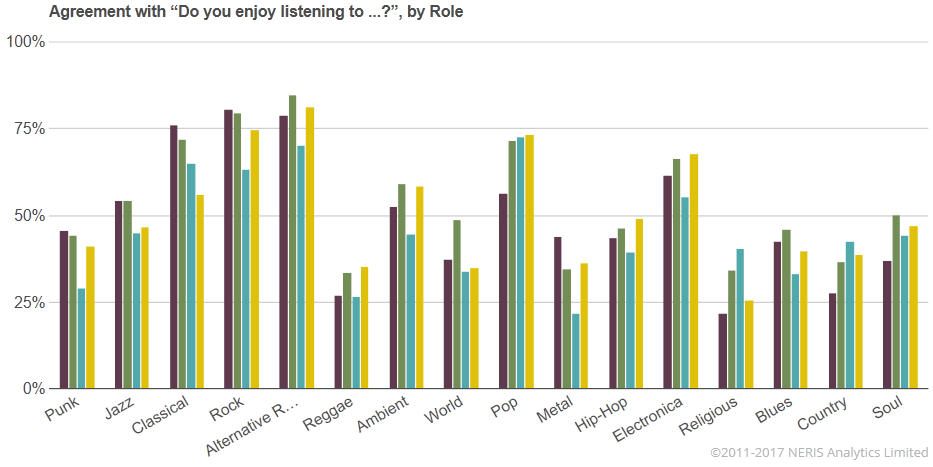
\includegraphics[scale=0.5]{survey_histogram.png}
\caption{Brown, green, blue and yellow bar represent respectively: Analysts, Diplomats, Sentinels, Explorers.}
\end{figure}

I have reported the results into a table in order to better classify Roles and their musical preferences. This allowed me to easily link each Myers-Briggs Type Indicator predicted by \textit{Apply Magic Sauce} with a relative vector of musical genres. 


\chapter{Implementation}

\section{Introduction}

In this chapter I will explain in details how the chatbot works, what happens under the hood from a technical perspective when users starts the conversation with the chatbot. The description will follow the usage flow of typical experience with the application.

\section{Initial phase}

The first interaction with the bot can occurs in two different ways: users can type his name in the search field of the different supported platforms or can follow a link that redirects them properly. All the platforms share a common paradigm to start a conversation that consists of sending a welcome event to Dialogflow, which triggers the entry point intent called \textit{Default Welcome Intent}; this is configured so that the response is not managed directly by Dialogflow but instead, is delegated to the webserver which pointer is configured as the default Dialogflow webhook for fullfillment option. A JSON object, containing information on the triggered intent, the resolved query, the sessionId, the timestamp, the language used, the status of the HTTP response and the original request, is sent to the webserver which parses it and according to the triggered intent, generates the response that is sent back to Dialogflow and so to the user on the messaging platform. When the webserver receives a \textit{Default Welcome Intent}, it checks if the user has already used the application before: the check is performed looking for a match between the user's platform id parsed from the JSON received by Dialogflow and the ones already in the database. In case of a positive outcome, the user is recognized and the message \textit{Happy to see you again <username>! To start, press the "Continue" button below!} is returned as a response.

\begin{figure}[ht]
\centering
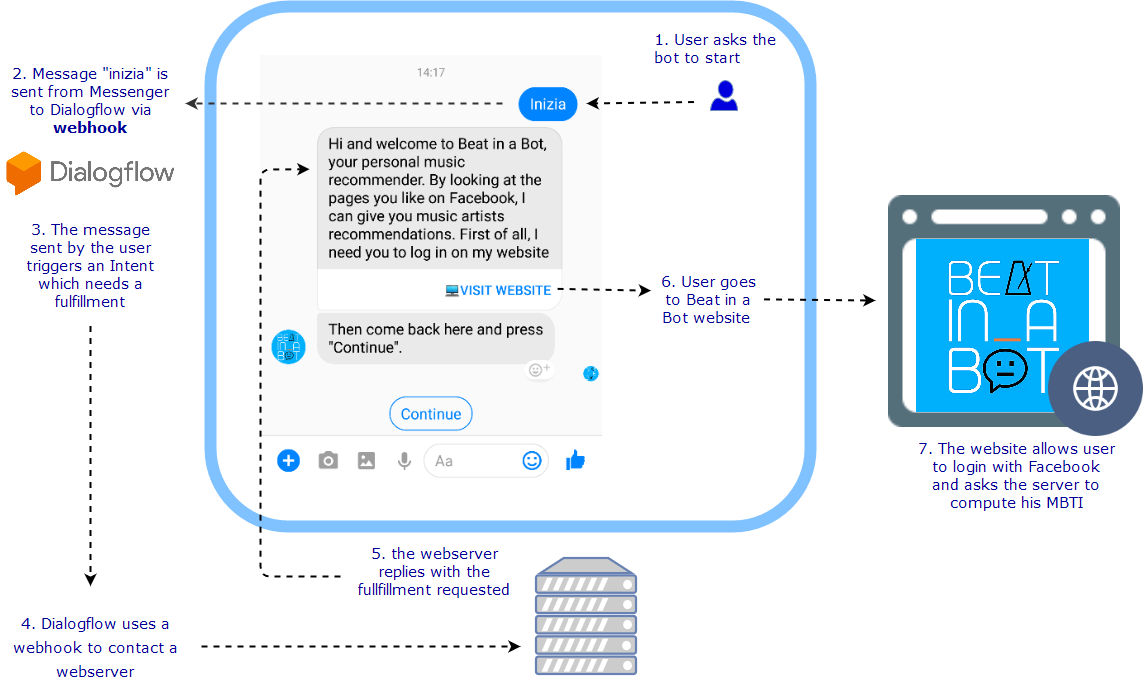
\includegraphics[scale=0.32]{workflow_start.png}
\caption{The initial workflow.}
\end{figure}

\section{Authentication}

Before moving on, I have to explain how users' authentication has been implemented. Users are identified with three different identifiers, the id assigned by the chat platform, the session id assigned by Dialogflow and his Facebook user id taken from the Facebook Login system on the external website. The reason of using such set of identifiers, is due to a lack of an integrated and shared way among all platforms, to authenticate a user. Each of the three ids has its own purpose: the session id, contained into the JSON from Dialogflow to the webserver, is active for 10 minutes and it is used to recognize a user among all the different requests in the same chat session; the platform id, also embedded into the JSON object, is used to identify the user on a specific platform and since it doesn't expire like the session id, it can be used as his main identifier (the one that makes possible to recognize him at the first interaction with the bot). The last id, the one returned when the user logs in with Facebook Login, is always unique regardless of the chat platform, thanks to the fact that the login operation is performed on an external website: this ID, being independent of the chat platforms and Dialogflow, is used to associate all the others to the same user so that he can be recognized among all the chat platforms.
\\
\noindent

While some platforms provides a webview as an integrated messaging chat element but others don't, in order to maintain compatibility with as much platforms as possible, the access to the login website is provided with a chat button which have as pointer, a customized Unique Resource Locator for each client. The link is built with the user's session id and a pointer to the bot, on the platform it has been opened, as query parameters; the session id is simply sent back to the server after the Facebook Login phase and has the purpose of linking the external website session to a specific user while the pointer to the bot, is needed to provide a back button after a successful login.

\begin{figure}[ht]
\centering
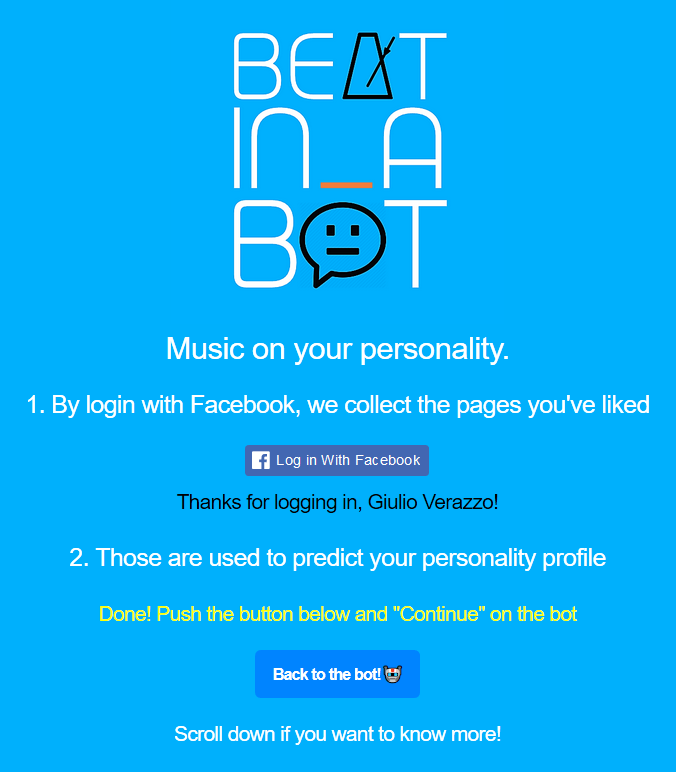
\includegraphics[scale=0.55]{website1.png}
\caption{The supporting website.}
\end{figure}


\section{Website implementation}

\subsection{Technical aspects}
The supporting website is developed using modern technologies for web developing like HTML5, CSS3, JavaScript and the JQuery library; rationale of choice is that these technologies are largely used by the web developers community and this represent added value in terms of technical support. The site is built upon a template by HTML5 UP  \citep{html5up} which provides free, customizable and fully responsive templates for the web. This allows me to have a web site that adapts easily on the different form factors of the screens of smartphones and tablets as well as desktop and notebooks. As for the hosting, I decided to use GitHub Pages   \citep{githubpages}, a service that gives the opportunity to host directly from the GitHub repository for free. From what regards developing details, I used Facebook JavaScript SDK to implement Facebook Login authentication system and the JQuery library to make an asynchronous GET request to the server. 

\subsection{Working logic}
When user clicks on the website button provided by the chatbot, a new window is opened and the page layout appears on the screen. The website is structured as a list of instructions to follow in order to log in and start the calculation of user's personality. The login functionality is implemented with Facebook Javascript SDK which, in order to be used, requires a registration on Facebook Developers portal. The registration is free and allow developers to create apps that can exploit Facebook services; when an app has been created, an app id is assigned to it. The app id must be inserted in the appropriate field of the SDK used; in this case, the Javascript SDK, which is asynchronously loaded inside the HTML page, provides a class called \textit{FB} which has a method, \textit{FB.init()}, that takes the app id as a parameter. After the SDK initialization, a "Log in with Facebook" button can be added to the page. The SDK automatically handles the login system and the user's login status. To access user's likes to Facebook pages, a special permission needs to be asked during the login phase: to make this permission asking possible, developers must submit the app to a verification process that requires two days to be completed: if the app has all the requirements an passes a Facebook internal test, the \textit{user\_likes} permission can be finally asked when users logs in. 
\\
After the user logs in, the website receives from Facebook an access token, that can be used to retrieve user's information from the Facebook Graph then, when user press the "Start!" button, the website asks the server to compute user's Myers-Briggs Type Indicator: this is done with a GET HTTP request, made with jQuery, that contains the following parameters: the Facebook user ID, access token and username and the Dialogflow session id. At this point, the server receives the request and proceed to check if user is already in the database: if it is, it directly replies with the JSON object taken from Apply Magic Sauce, if is not, using the access token, it first sends a request to the Facebook Graph in order to retrieve the list of user's likes to pages and then, sends it to Apply Magic Sauce. The response received is a JSON object that contains values expressed in percentile of the Big 5 factors, the user's Myers-Briggs Type Indicator and the sets of pages that has determined, in a positive or negative way, each value of the Big 5 traits. The JSON object, together with user's MBTI, Facebook id, username and the session id are stored to the users table of the database and finally the webserver replies to the original website request, with the JSON object from Apply Magic Sauce.
When the website receives the response, the "Start!" button disappear and a "Back to the Bot!" button takes his place; such button has the purpose of creating a natural flow that guides the user from the website back to the chatbot after the login phase. Its implementation depends on the chat platform used to talk with the bot: if Telegram, the button just points to an \path{http://t.me/<botname>} link, if Messenger, since the website appears inside a webview within the chat, it needs a proper method of the Facebook Messenger SDK to be closed.
\\
After setting the back button, the website parses the JSON object received and calls two methods: \texttt{JungianTypeResult(mbti)} and \texttt{showLikes(obj, mbti)}. The former takes the Myers-Briggs Type Indicator read from the JSON and populates an empty DIV with a brief description of the indicator taken from the official Myers-Briggs Foundation website   \citep{MBfoundation} and a picture of a famous musician with the same personality as the user   \citep{Intuitivemusician}; the latter converts the Big 5 dimensions to MBTI dimensions and builds a table, which rows, are populated with the pictures of the Facebook pages that has determined the four dimensions of user's personality.

\begin{figure}[ht]
\centering
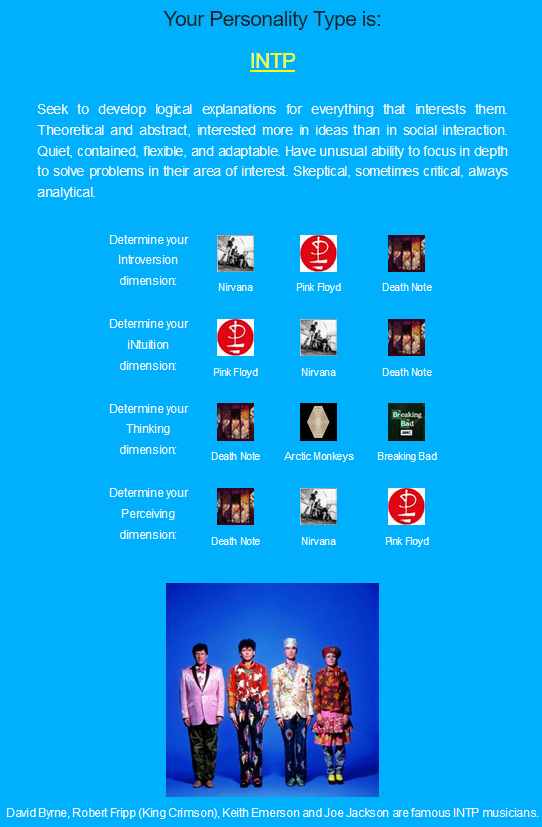
\includegraphics[scale=0.59]{website2.png}
\caption{Additional information on user's personality.}
\end{figure}


\pagebreak

\subsection{MBTI - BIG5 Conversion}

To show users which Facebook pages determine the four dimensions of their Myers-Briggs Type Indicator, a conversion to the Myers-Briggs domain of the Big 5 index values returned by Apply Magic Sauce, is required. Such conversion is based on a study   \citep{big5-mbti} by McCrae \& Costa who had the purpose of reinterpreting the Myers-Briggs Type Indicator from the perspective of the Five-Factor Model of personality. The study was conducted by submitting a sample of 267 man and 201 women, ages 19 to 93, to both the NEO-PI (the standard Big 5 inventory) and the MBTI inventory with the aim of finding a correlation between the indices of the two models. The correlational analyses showed that the four MBTI indices did measure aspects of four of the five major dimensions of normal personality: in particular, a negative correlation was found between the Big 5 Extraversion factor and the Extraversion-Intraversion factor of MBTI scale, same for Big 5 Conscientiousness and the Judging-Perceiving factor, while a positive correlation showed up between Big 5 Openness and the MBTI Sensing-iNtuition and between the Big 5 Agreeableness and the Thinking-Feeling factor of MBTI. As for the Neuroticism factor, no significant correlation result was found.

\begin{figure}[ht]
\centering
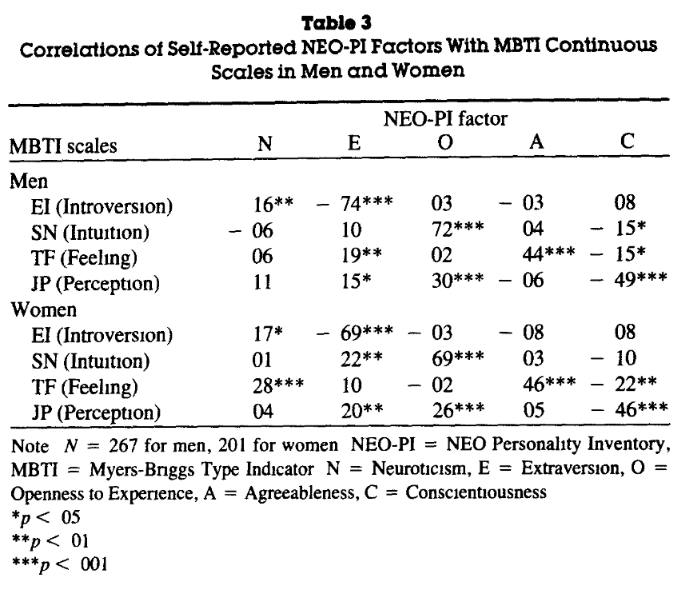
\includegraphics[scale=0.68]{big5-mbti.png}
\caption{Correlations of Self-Reported NEO-PI Factors With MBTI Continuous Scales in Men and Women}
\end{figure}

\section{Second phase: personality and recommendations}

When the bot acquires the focus again after pressing the \textit{Back to the bot!} button on the website, the next step consists of sending the keyword \textit{Continue} to the bot with the provided \texttt{quick reply} button. Quick replies are in-conversation buttons that appear prominently above or inside the composer; when a quick reply is tapped, the buttons are dismissed, and the title of the tapped button is posted to the conversation as a message. This particular design solution founds his meaning to the fact that Dialogflow doesn't allow bots to send a message that isn't a reply to a user's previous message. 

\begin{figure}[ht]
\centering
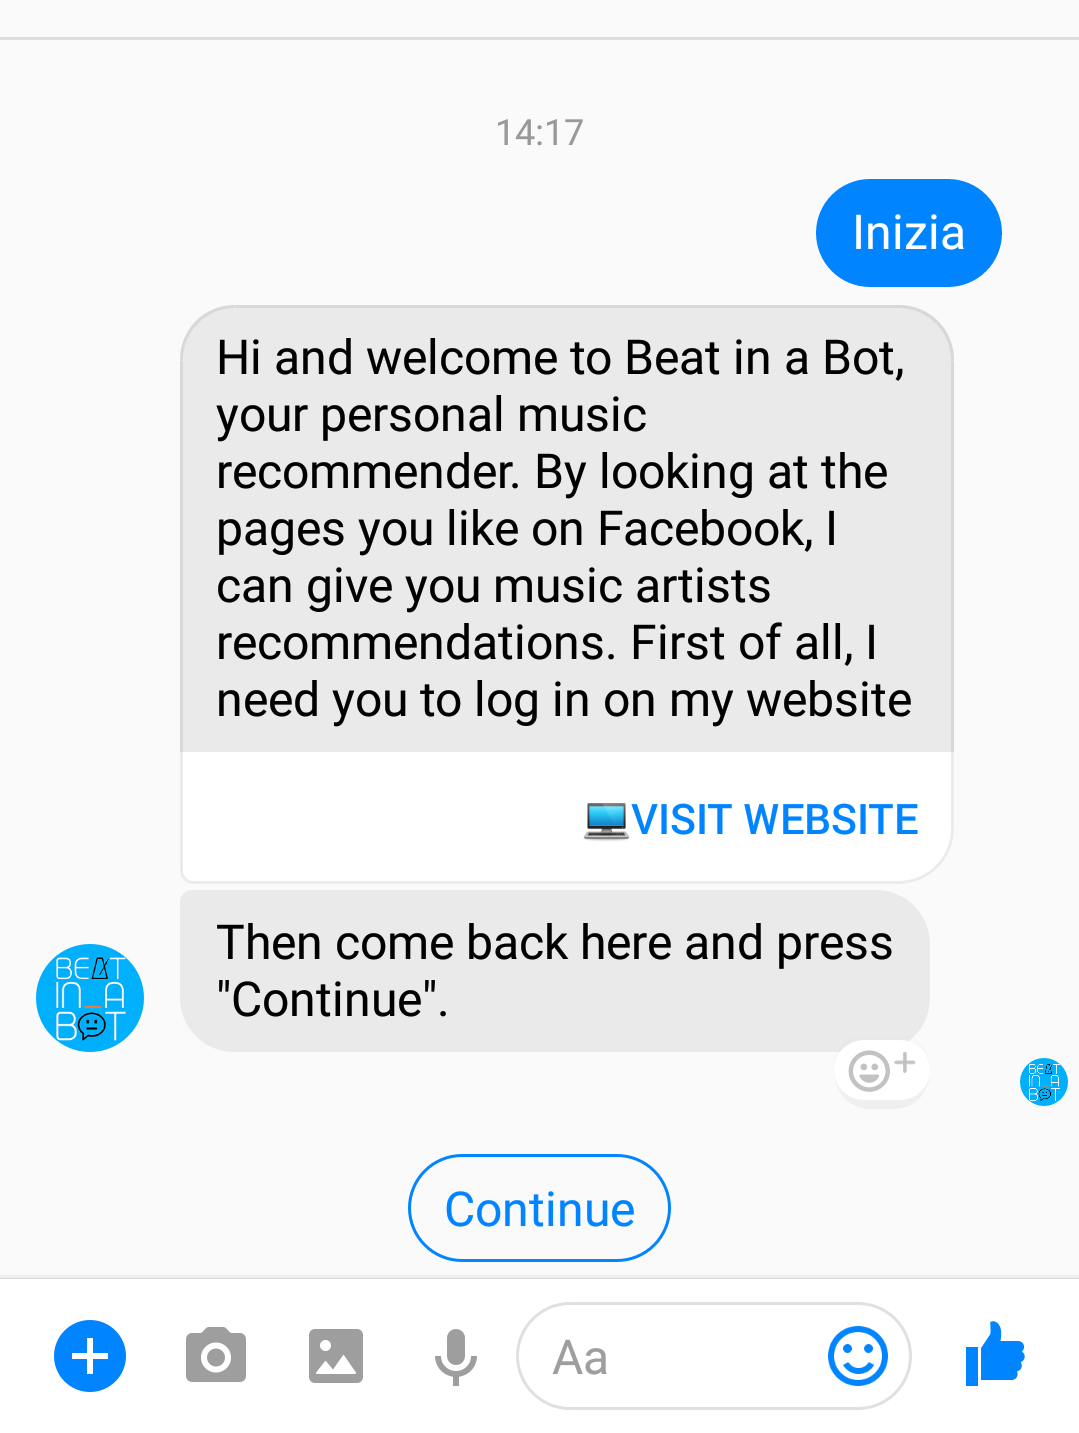
\includegraphics[scale=0.2]{bot_start.png}
\caption{Bot onboarding message and quick reply button.}
\end{figure}

When the keyword is received by Dialogflow, it triggers an intent that sends an HTTP request to the server webhook. The server checks that the chat session id is in the database and from here, three possible scenario can occur:

\begin{enumerate}
    \item User has gone to the website, followed the instructions given and tapped on the quick reply button.
    \item User has tapped the quick reply button without first visiting the website or has wrote something unexpected to the bot.
    \item User has gone to the website and then has wrote something unexpected to the bot.
\end{enumerate}

\noindent
On the first scenario, the conversation follows its natural flow and the message \textit{"Cool! Your Facebook digital footprints tells me that you are an <MBTI> person. Do you want to know more about your personality or go straight to your music recommendations?"} is returned as a positive outcome by the webserver.

\begin{figure}[ht]
\centering
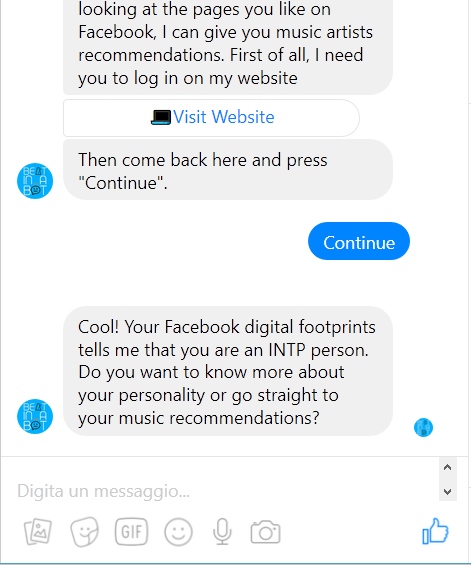
\includegraphics[scale=0.7]{bot_positive.png}
\caption{First scenario.}
\end{figure}

\noindent
Users can reply with open phrases like \textit{"Tell me more about my personality"} or \textit{"Recommendations please"}. Association between open phrases and intents is managed by Dialogflow with a proprietary Natural Language Processing algorithm that mixes a rule-based approach with a machine learning model   \citep{dialogflowML}. Based on the response given by the user, either the \textit{Personality - more} intent or the \textit{Recommendation} intent can be triggered: in the first case, response is given by the webserver which replies with the same description of the user's Myers-Briggs Type Indicator shown on the website and a quick reply button with the text \textit{"Now recommend me!"}. In the other case, the webserver computes the recommendations and replies with the first artist's card. Details on how recommendations are built will be explained in a following section.

\pagebreak

\begin{figure}[ht]
\centering
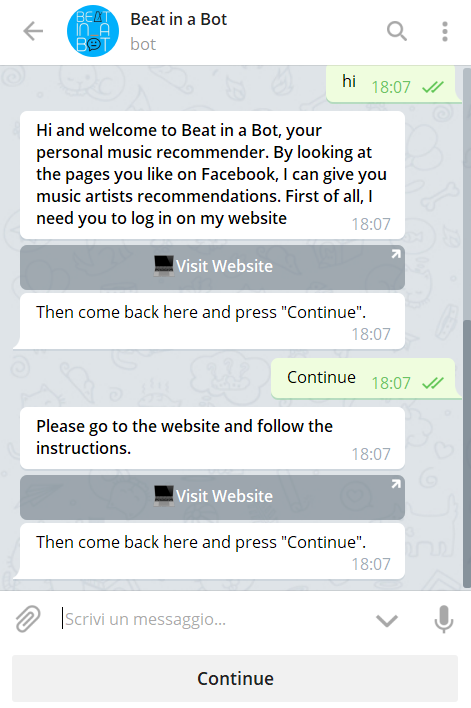
\includegraphics[scale=0.6]{bot_error.png}
\caption{Second scenario.}
\end{figure}

On the second scenario, that occurs when user has tapped the quick reply button without first visiting the website or has wrote something unexpected to the bot, the conversation breaks and instructions on how to proceed correctly are given to the user. Instructions includes a text message, a new button to the website and a new \textit{"Continue"} quick reply button.
\\
\\
The third and last scenario is managed by Dialogflow using the \textit{Fallback Intent} option. Fallback intents are triggered if a user's input is not matched by any of the regular intents; the conversational flow is built setting the output and input contexts of the various intents properly and fallback intents follows the same rule. In this particular case, the \textit{Personality} intent, that is triggered by the \textit{"Continue"} keyword, has the \textit{personality} context both as input and output context and the \textit{recommmendation} context as additional output context. If no user's input matches the \textit{Personality} intent, its relative fallback intent, that has \textit{personality} as input context, triggers and the response is delegated to the webserver which replies with the message \textit{"It's not so hard, just push the continue button below."} and the \textit{"Continue"} quick reply button to recover from the error.

\begin{figure}[ht]
\centering
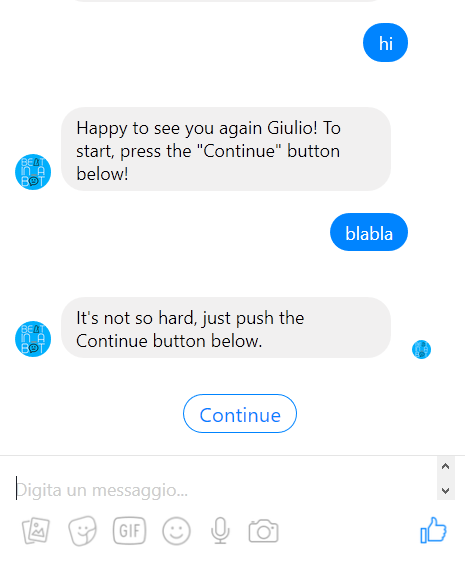
\includegraphics[scale=0.7]{bot_error2.png}
\caption{Third scenario response.}
\end{figure}

\section{Recommendations}

The recommendations phase starts when the user ask the bot to compute them: this triggers the \textit{Recommendation} intent inside Dialogflow and the response is once again built by the webserver. Using the session id as a key, the webserver extract the user's MBTI from the database and passes it as an argument to the function \texttt{genresListFromJungianType(...)}. The function returns a list whose elements are the musical genres associated to the given MBTI by the study conducted by NERIS Analytics Limited   \citep{survey}. Next, the server calls the \texttt{artistsIDsFromFile(...)} method which takes the user's Facebook id and his MBTI as arguments and implements the following value chain:

\begin{figure}[ht]
\centering
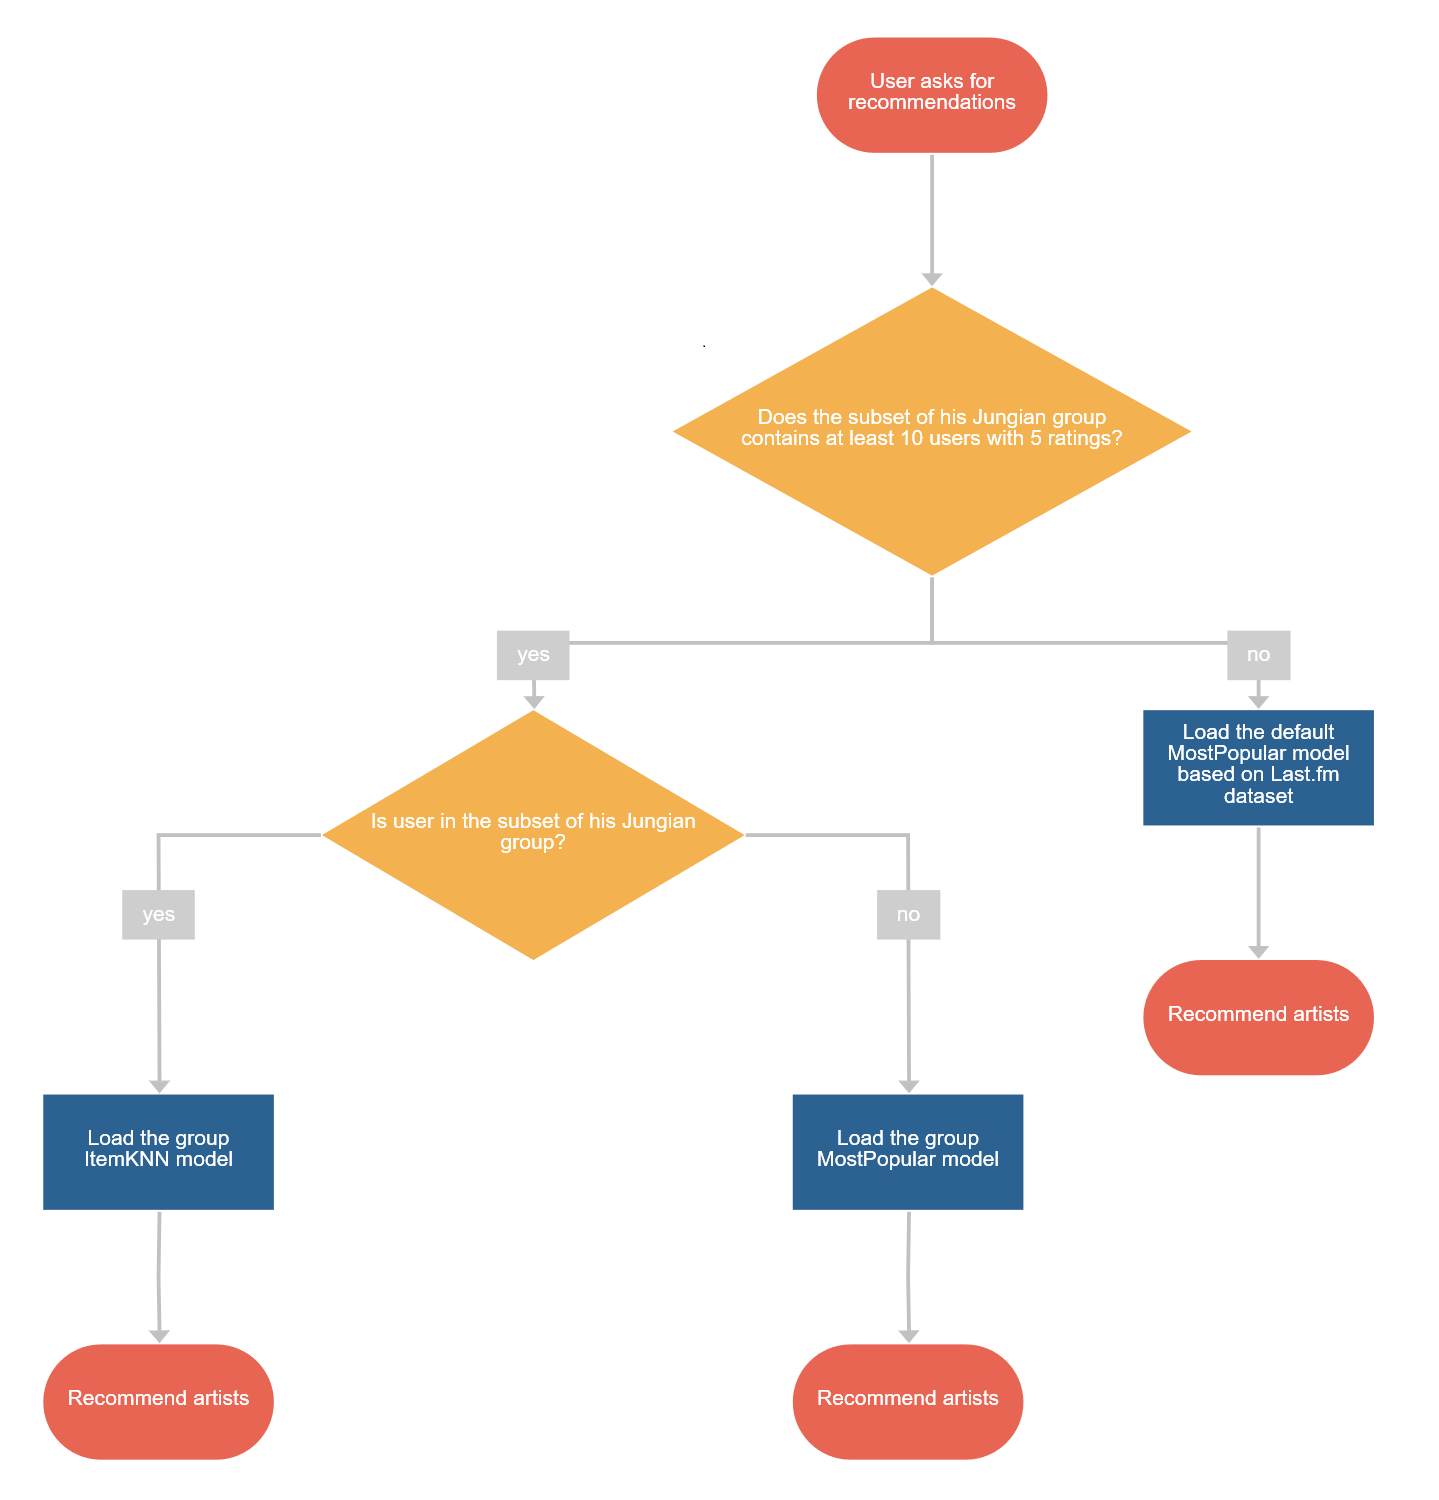
\includegraphics[scale=0.37]{value_chain.png}
\caption{The value chain of Beat in a Bot recommendation process.}
\end{figure}

\subsection{Recommender models generation}

Before moving on with the details of the value chain, it is necessary to explain how the recommender system works. As written in the approach section, the recommender system used is \textit{MyMediaLite}. MyMediaLite is released as a binary file which can be executed from the command line passing a set of arguments that specifies the possible operations available. The binary file is programmatically executed using the \texttt{Popen(...)} method of the \texttt{process} library for Python. The recommender system executable is mainly used for two operations: to save recommender system models and to load the models for prediction making. The first operation is executed by a Python script that is programmed to run every 30 minutes using the Unix command cron. Cron is a Unix utility that allows tasks to be automatically run in the background at regular intervals by the cron daemon. The tasks, called \textit{cron jobs} are written into a file called \textit{CronTab} which contains the schedule of cron entries to be run and at specified times. The application cronjob creates four CSV (Comma-Separated Values) files that contains the user-likes entries of the four personality groups and an additional CSV file of the user-likes entries of all the users in the database. Those files are used to generate the prediction models for both the MostPopular and the Item K-Nearest Neighbour algorithms; the result of this operations consists of nine files: four Most Popular models of the personality groups, one Most Popular model for all the users and four ItemKNN models of the personality groups.
\\
To save models, the recommender system executable takes as input the CSV file of user's group, used to train the model, and generates as output, the model file. If no \texttt{--recommender} option is specified, the Most Popular algorithm is used by default. It runs with the following command:

\begin{verbatim}

./mymedialite/item_recommendation 
--training-file=mymedialite/data/<group_name>.csv 
--save-model=mymedialite/models/<group_name>_MPmodel

\end{verbatim}


\subsection{Recommendation value chain}

The idea behind the recommendation process is to give users the best recommendations possible based on the data available on his ratings. Since users' personalities are grouped into four categories, the first decision process is taken on the amount of groups user-likes data available in the database: if data on the group from which the user belongs to are enough, i.e. there are at least 10 users which of them has given at least 5 ratings, the algorithm proceeds with a second decision process otherwise, it loads the Most Popular model file based on the Last.fm dataset, which can be used to predict general recommendations. The second decision process checks if the active user is part of the user-likes data of his group. If so, it means that there is a user history and so, the ItemKNN model can be loaded and used: this allows to find the recommendations with the highest precision possible. If the user is not part of the user-likes data, means that he is a new user and he will be present when the next cron job executes; in this case, the personality group Most Popular model is loaded and used to predict optimal recommendations.
\\
Recommendations prediction is executed running MyMediaLite with the following command:

\begin{verbatim}

./mymedialite/item_recommendation 
--training-file=mymedialite/data/<group_name>.csv 
--load-model=mymedialite/models/<group_name>_ItemKNNmodel  
--prediction-file=mymedialite/mml_output/<fbuserid>.prediction

\end{verbatim}

\noindent
It takes three arguments: the training file used to train the model, the model that has to be used to make predictions and the name of the output prediction file. As a design choice, every prediction file is named with the active user's Facebook id in order to be unique for each user.
\\
When the webserver receives the request by Dialogflow with \textit{Recommendation} as the triggered intent, it calls the method \texttt{artistsIDsFromFile(...)} which reads the output prediction file of the active user and returns a list with the artists ids predicted for him. At this point, for each user's favourite music genres, 50 artists are extracted from the database and inserted in a temporary list. Such list is shuffled to add some randomness to recommendations, then the first two artists are taken from the list head and pushed in the user's recommendations list. At each iteration, the algorithm checks if there are doubles in the recommendations list and removes it. When the loop ends, the list is first reversed and then inserted as a JSON object in the relative user's row of the database. The solution of reverting the list is due to the fact that recommendations are given with stack logic. This derives from the way recommendations are presented to users in the chatbot interface: it shows one artist recommendation at a time, in a form of a card containing the artist name, his music genre, an image taken from his Last.fm profile and two buttons \textit{Next} and \textit{I like it!}: the first is used to navigate recommendations and the second to express a preference. The logic behind the operation of the \textit{Next} button is as follows: when the button is pressed, the \textit{Next} intent is triggered in Dialogflow and the response managed by the webserver as usual. The webserver takes the user's recommendations reversed list from the database, pops out the next recommendation and puts the list back into the database; this logic provides a natural way to take the count of recommendations in order to signaling the user when they are over.

\newpage

\subsection{User preferences}

Users can express their positive-only feedback tapping the \textit{I like it!} button above the artist's card. Each like button is built to send a special string as postback to the bot. Such string is encoded as follows: \texttt{"id=<artist\_id> fbuserid=<user\_id>"}. An intent named \textit{like} inside Dialogflow, is triggered only by this specific string and the two ids contained are catched as system entities. As a consequence, the two values will take a dedicated space in the JSON object sent to the webhook. When the webserver receives the request from Dialogflow, the two ids can be easily read parsing the JSON object.


\begin{figure}[ht]
\centering
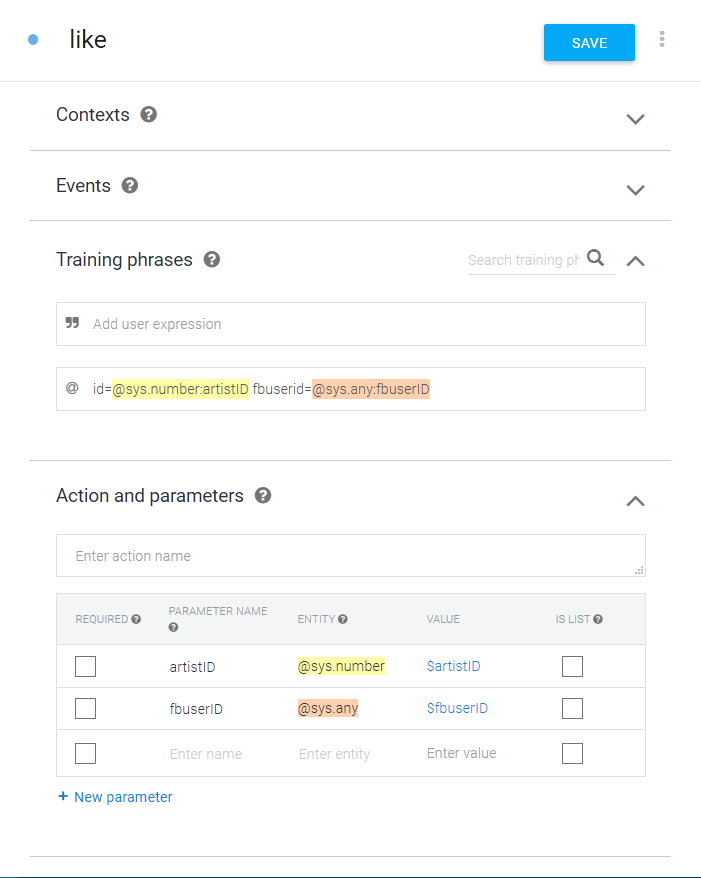
\includegraphics[scale=0.5]{DF_like_intent.png}
\caption{The like intent inside Dialogflow}
\end{figure}

\pagebreak

\noindent
At this point, the webserver stores the user feedback in the database and replies with a text, randomly chosen from a list of variants, and a quick reply button \textit{"Next artist"} that guides the user in the bot interaction. 

\begin{figure}[ht]
\centering
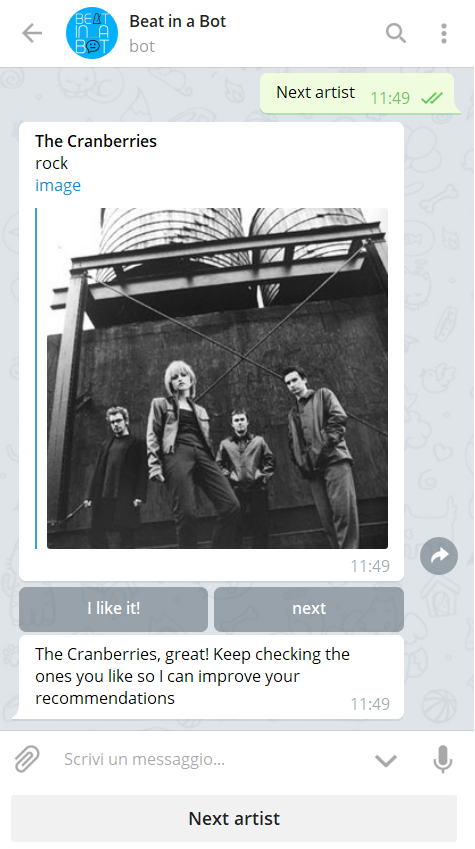
\includegraphics[scale=0.71]{bot_likeit.png}
\caption{Bot response to user feedback}
\end{figure}

\newpage

\noindent
If the user writes something unexpected to the bot, a fallback intent named \textit{next - fallback}, entirely managed by Dialogflow, triggers and instructions for error recovering are given to the user.

\begin{figure}[ht]
\centering
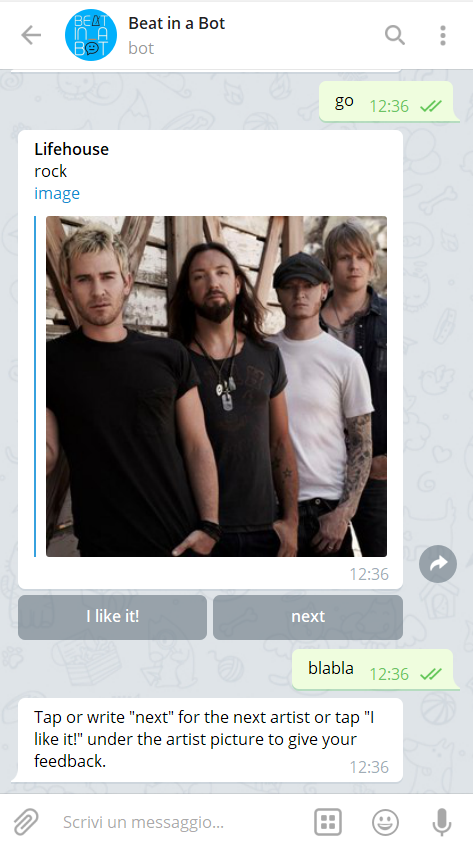
\includegraphics[scale=0.71]{bot_next_error.png}
\caption{Bot response to unexpected input during recommendations phase}
\end{figure}


\chapter{Experimental validation}
%Analytics-Utility-Usefulnes
\section{Introduction}

This chapter is dedicated to an experimental validation of the chatbot application developed. The validation is composed by three different tests: a design test, an usability test and an usefulness test. The design of the application has been tested with online tool called Alma, the chatbot test. It is based on a heuristic evaluation of 7 metrics of chatbots design. A test reliability study has been conducted to validate the tool. The application usability has been tested with a qualitative survey based on Nielsen's heuristics; this subsection includes a background and an analysis of the test results. The utility of the application was evaluated with an experiment: it have been asked to 43 people to use the bot and to mark their preferences on recommendations considered interesting. The subsection contains an analysis of the results obtained. 


\section{Design test}

\subsection{Introduction}

To test chatbot design an online tool called \textit{Alma}   \citep{chatbottest} has been used. Alma is a free Chrome extension released as an open source project by Jesús Martín (Product Designer for BEEVA Labs), Carlos Muñoz-Romero (Digital Product Manager for monoceros.xyz) and Nieves Ábalos (Conversational Interfaces expert for monoceros.xyz) that acts like a chatbot itself. Alma asks 33 questions that helps to find problems in the human-chatbot interaction. The test is based on a heuristic evaluation of 7 metrics of chatbots design:

\begin{itemize}
    \item Personality: Alma's questions tries to understand if the chatbot has a clear personality any user would recognize as unique; if that personality is consistent on the whole conversation; if it is appropriated for the users that will use the chatbot; and last but not least if the tone can be readapted according to the ongoing conversation.
    
    \item Onboarding: Users are gonna arrive from all over the world, with different levels of expertise about how to use a chatbot, and with different expectations of what our chatbot can do. Making clear what is the chatbot capable to do, and how users can get the most of it, it’s crucial to avoid errors and frustration.
	
	\item Understanding: Testing the understanding of a chatbot is something that mainly deals with technical aspects of the development. This part really depends on the type of service the chatbot is giving: if it pretends to be a human-like experience, the level of understanding must be high, otherwise a command based conversation is acceptable if the bot is mainly a single purpose service.
	
	\item Answering / Speaking: Chatbot speaking used to be based on plain text, but now we are very far from that. The problems associated with NLP, and the real capability of technology understanding what users are writing is changing the game. The situation has filled conversational interfaces with a lot of different interaction elements, so the aim of any question here is to find out what elements does the chatbot send and how well it is doing it. 
	
	\item Navigation: In a conversational interface there are no breadcrumbs, back buttons or a search box to help users go from some parts of the interaction to others. However, users have the same needs they used to have with traditional interfaces: they change their mind and want to go back, they want to skip steps. Conversation is creating its own methods to deal with some of these needs and testing how well your chatbot is doing it is something really important.
	
	\item Error management: Technology is still not able to understand most of what users are asking to chatbots and the interactions between the two of them are far from being perfect. Having that certainty in mind, chatbots need to be prepared whenever the error happens with different strategies to repair the situation.
	
	\item Intelligence: The test includes some questions that tries to find the ability of a chatbot to know things not necessarily said by the user, remember others that appear during the interaction, and use that knowledge to adapt the conversation to the user and the specific situation.
\end{itemize}
\pagebreak
\subsection{Design test results}

Test results are presented in a circular diagram in which each of the seven metrics is expressed in a range between 0 and 100.
Beat in a Bot design test has given the following results: 

\begin{figure}[ht]
\centering
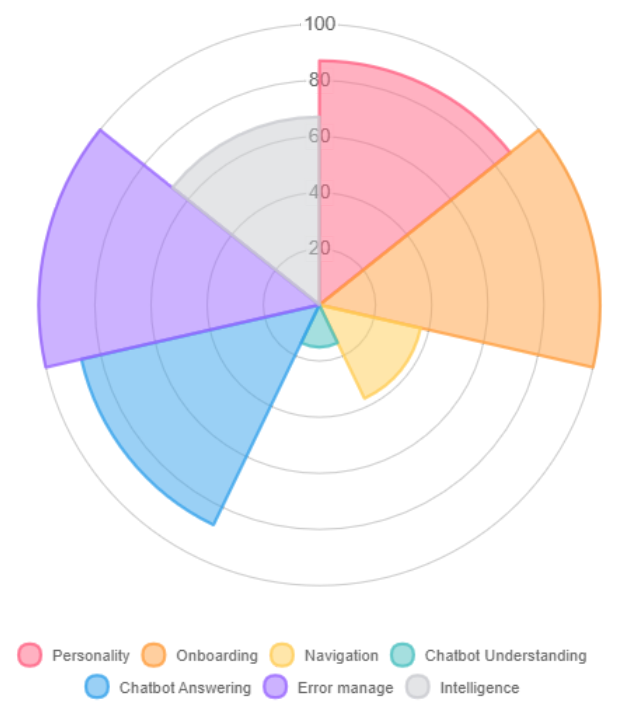
\includegraphics[scale=0.5]{chatbottest.png}
\caption{A circular diagram reporting the scores of each metric of the test results.}
\end{figure}


Before analyzing the test results, it's necessary to have in mind that there is a difference in the weight of the metrics values, depending of the type of bot being tested. For instance, for a bot that has the purpose of entertaining a human-like conversation with the user, the "Chatbot Understanding" metric has particular importance that for a single-purpose bot. As for the former, it is expected to answer to a large set of questions about different topics, but for the other, users only expect it replies to questions about his mainly activity.

\subsubsection{Personality} As for the personality of the chatbot, the score marks a value between 80 and 100, indicating a recognizable "persona". The bot tends to maintain the same tone during the conversation and always responds consistently with what is asked over time. Furthermore, the answers are always relevant, in the sense that, they reflect user's expectations.

\subsubsection{Onboarding} Onboarding scores a mark of 100. The chatbot greets the user as soon as he writes the first message explaining what it his purpose and giving the instruction on how to continue the interaction.

\subsubsection{Navigation} Navigation scores a mark just below 40. The reason is that, the chatbot, because of the nature of the service he offers, does not need to provide the user with options to undo operations since there is no critical task that needs to be undone (like for instance, online shopping bots).

\subsubsection{Chatbot Understanding} Here the chatbot has his lowest score, under 20. As for the metric "Navigation" the reason for this result is due to the intrisic single-service nature of the bot, whose conversational interface is mainly command-based. It doesn't need to have a vast natural language understanding level, since available commands are presented directly to user from the bot; this is a design choice to make the conversational flow as effective as possible while reducing the risk of understanding errors.

\subsubsection{Answering/Speaking} The answering / speaking metric settles on an high value, between 80 and 100. The chatbot always gives the right answer to the given command and, once the onboarding process is completed, it shows a card-buttons interface that allows to navigate between recommendations, give a preference for an artist or visit his Last.fm profile (Figure 5.2).

\subsubsection{Error Manage} Test has given the mark of 100 for the "Error manage" metric. The bot correctly recognize and manage error cases and report instruction on how to continue. A representative example is the case in which the user tries to jump the log in phase. The bot acknowledge that and asks the user to please log in before continue with the conversation (Figure 5.3).

\subsubsection{Intelligence} Intelligence score a mark just above 60. Since the bot records the chat session and uses an authentication system, it has the ability to remember data and preferences not explicitly said by the user. Those are used to adapt the conversation to the user and to the specific situation, tailoring recommendations as preferences are expressed.

\subsection{Test reliability study}

Tests aim to measure dimensions (or factors) of constructs through indicators. It is known that every measurement brings errors that can be random or systematic. To keep incidence of errors under control, the concept of reliability is introduced. Reliability is the degree to which an assessment tool produces stable and consistent results i.e. the degree of coherence between independent measurements of the same construct. A measure is said to have a high reliability if it produces similar results under consistent conditions. 
\textit{Usability} is the construct of the test whose validity is to be measured and its indicators are:
\begin{enumerate}
\item Personality
\item Onboarding
\item Navigation
\item Chatbot understanding
\item Chatbot answering
\item Error management
\item Intelligence
\end{enumerate}

\noindent 
The \textit{reliability coefficient} of the test expresses the proportion of true variance in the measurement with respect to the total variance.

\begin{equation}
    r_{tt} = \frac{\sigma^{2} (V)}{\sigma^{2}(X)} = \frac{\sigma^{2} (X) - \sigma^{2} (E)}{\sigma^{2}(X)} = 1 - \frac{\sigma^{2} (E)}{\sigma^{2}(X)}
\end{equation}

The variance, expressed as $\sigma^{2}(X)$ measure how far a set of (random) numbers are spread out from their average value. It is an index of spreading. 
There are several methods to compute reliability of a test:

\subsubsection{Test-Retest Method}
The Test-Retest method is the simplest way of testing the stability and reliability of an instrument over time. Consists of submitting the test at two different times, T1 and T2, and then calculate the correlation between the two scores. This method relies upon the calculation of the Pearson correlation coefficient.

\subsubsection{Parallel-forms method}
The Parallel-forms method consists of submitting two equivalent version of the test (same average and same standard deviation) , to calculate then, the correlation between values of the two forms as an evaluation of reliability.

\subsubsection{Split-half method}
The Split-half method consists of first submitting the test once, then subdivide the test in two equal halves and consider them as two parallel-forms (same average and same standard deviation). The reliability is then calculated as a correlation between values of the two forms.

\subsubsection{Internal coherence method}
The internal coherence test consist of submitting the test only once, at time T1. Each item is considered as a separate test. The average correlation between all the items is estimated (with special formulas), and from it, an evaluation of the reliability coefficient is derived.

\subsection{Reliability test and results}

The method chosen to evaluate the reliability of the chatbot design test is the Test-Retest method because it's the only one that doesn't require additional work on the test itself: the test is made by external source and there's no way to subdivide it into two equal halves; furthermore, there is no equivalent test available that can be used as a different form.
The following table shows the values of the indices obtained in the two tests taken at time T1 and T2:
\pagebreak

\begin{table}[]
\centering
\begin{tabular}{|l|l|l|l|}
\hline
\multicolumn{2}{|l|}{}                          & \textbf{T1 (01/25/2018)} & \textbf{T2 (02/5/2018)} \\ \hline
\multicolumn{2}{|l|}{\textbf{Personality}}      & 82                       & 79                      \\ \hline
\multicolumn{2}{|l|}{\textbf{Onboarding}}       & 100                      & 100                     \\ \hline
\multicolumn{2}{|l|}{\textbf{Navigation}}       & 38                       & 40                      \\ \hline
\multicolumn{2}{|l|}{\textbf{Understanding}}    & 16                       & 22                      \\ \hline
\multicolumn{2}{|l|}{\textbf{Answering}}        & 82                       & 87                      \\ \hline
\multicolumn{2}{|l|}{\textbf{Error management}} & 100                      & 100                     \\ \hline
\multicolumn{2}{|l|}{\textbf{Intelligence}}     & 64                       & 67                      \\ \hline
\multicolumn{2}{|l|}{}                          &                          &                         \\ \hline
\multicolumn{2}{|l|}{\textbf{Average}}          & 68,86                    & 70,71                   \\ \hline
\multicolumn{2}{|l|}{\textbf{Std. deviation}}   & 29,41                    & 27,72                   \\ \hline
\end{tabular}
\end{table}

\noindent The test-retest coefficient is calculated with the following formula:

\begin{equation}
r_{tt} = \frac{Cov (T1,T2)}{Dev.St(T1) \ast Dev.St.(T2)}
\end{equation}

\noindent The covariance is equal to:

\begin{equation}
Cov(T1,T2) = 812,53
\end{equation}

\noindent The test-retest coefficient is equal to:

\begin{equation}
r_{tt} = 1
\end{equation}

\subsection{Result analysis}
\noindent The test-retest reliability coefficients (also called coefficients of stability) vary between 0 and 1, where:
\begin{itemize}
\item 1 : perfect reliability,
\item >= 0.9: excellent reliability,
\item >= 0.8 < 0.9: good reliability,
\item >= 0.7 < 0.8: acceptable reliability,
\item >= 0.6 < 0.7: questionable reliability,
\item >= 0.5 < 0.6: poor reliability,
\item < 0.5: unacceptable reliability,
\item 0: no reliability.
\end{itemize}

On this scale, a correlation of .9(90\%) would indicate a very high correlation (good reliability) and a value of 10\% a very low one (poor reliability). The result obtained with the test-retest method taken to evaluate the reliability of thechatbottest.com, is a reliability coefficient equal to 1: this indicates a perfect reliability of the test.

\section{Usability test}

The application usability test has been carried out following the experiment conducted to measure its usefulness. To each experiment attendant, it has been asked to fill a survey of 9 questions, based on a custom review of Jakob Nielsen's usability heuristics for evaluating user interfaces. Jakob Nielsen, Ph.D., is a User Advocate and principal of the Nielsen Norman Group which he co-founded with Dr. Donald A. Norman (former VP of research at Apple Computer). Nielsen established the "discount usability engineering" movement for fast and cheap improvements of user interfaces and has invented several usability methods, including heuristic evaluation. He holds 79 United States patents, mainly on ways of making the Internet easier to use. In 1995 he developed 10 usability heuristics    \citep{Nielsen} for evaluating user interfaces. These heuristics have stood the test of time, providing designers with a quick and easy way of evaluating the usability of software interfaces against a set of universal design principles.

\begin{figure}[ht]
\centering
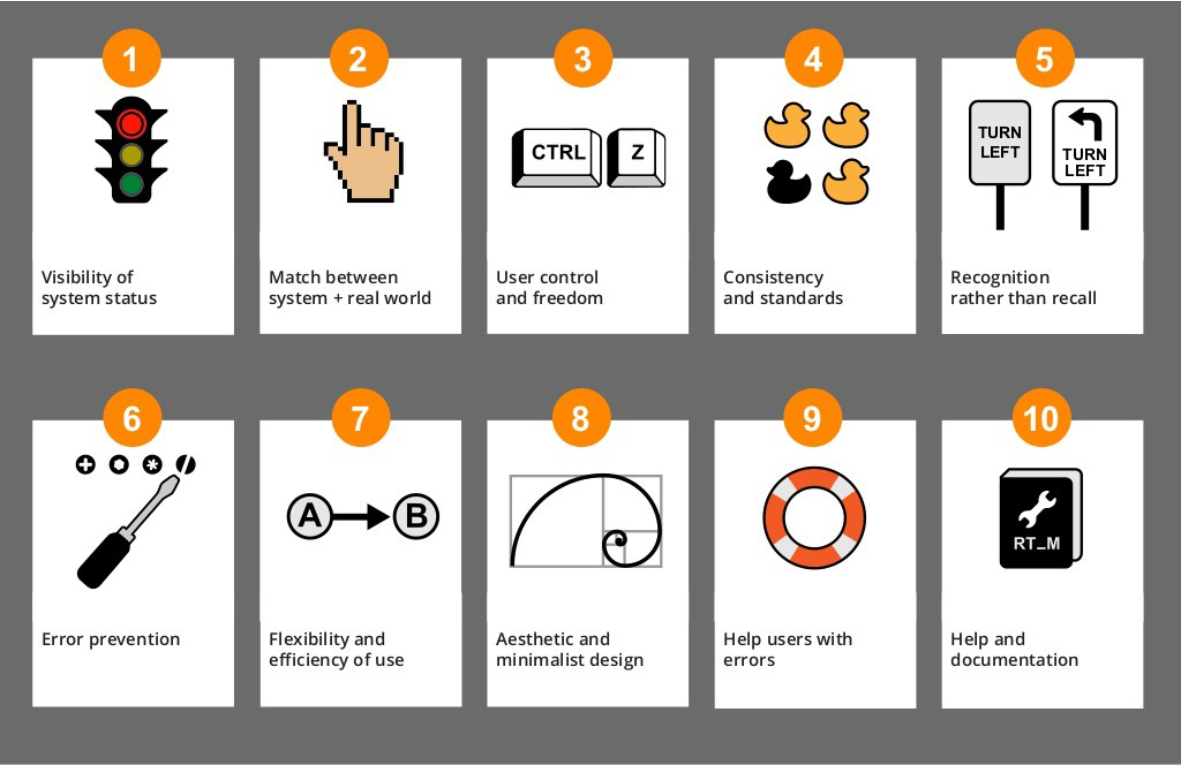
\includegraphics[scale=0.4]{nielsen_heuristics.png}
\caption{Nielsen's Ten Heuristics.}
\end{figure}

\subsection{Nielsen's Ten Heuristics.}
This subsection reports the Nielsen's ten heuristics for user interfaces and for each of them, an analysis is done to adapt them to the world of chatbots.

\subsubsection{1. Visibility of system status}
\textit{"The system should always keep users informed about what is going on, through appropriate feedback within reasonable time."}
\\
\\
The medium of bots is a conversation, and conversation is governed by messages. Since message are ephemeral, they become stale with time and old messages are less valuable than one from few seconds ago. This heuristic can be ported to chatbots in a slightly different form: the system should allow the user to \textit{request} information about what is going on, through appropriate feedback within reasonable time.

\subsubsection{2. Match between system and the real world}
\textit{"The system should speak the users’ language, with words, phrases and concepts familiar to the user, rather than system-oriented terms. Follow real-world conventions, making information appear in a natural and logical order."}
\\
\\
The main obstacle to achieve this is that, despite chatbots are made to chat, they have problems with language understanding. Even those built atop the latest tech are limited in what they can understand and how well they can respond. The key to best follow this heuristic is to know the chatbot audience. Some users will appreciate a command line style interaction style, and others will expect to converse in natural language. Still others might speak in slang or abbreviations. Bots should be built with a solid understanding of the audience they seek to appeal to.

\subsubsection{3. User control and freedom}
\textit{"Users often choose system functions by mistake and will need a clearly marked “emergency exit” to leave the unwanted state without having to go through an extended dialogue. Support undo and redo."}
\\
\\
Chatbot can easily implement "emergency exits", keeping the user aware of valid options during any stage of an interaction.

\subsubsection{4. Consistency and standards}
\textit{"Users should not have to wonder whether different words, situations, or actions mean the same thing. Follow platform conventions."}
\\
\\
Unfortunately, at the time, there aren't platform conventions for chatbots but this heuristis can be interpreted to mean that bots should be internally consistent; a bot should stick to a single style of language, whether that’s natural language, command line, or something in between.

\subsubsection{5. Error prevention}
\textit{"Even better than good error messages is a careful design which prevents a problem from occurring in the first place. Either eliminate error-prone conditions or check for them and present users with a confirmation option before they commit to the action."}
\\
\\
Thanks to the conversational nature of chatbots, it's quite easy to follow this design principle.
Bot designers should build interactions with the assumption that errors will happen early and often, given the ambiguity and impreciseness of most human dialogue. Bots have to ask for confirmation from the user for any critical step in an interaction.

\subsubsection{6. Recognition rather than recall}
\textit{"Minimize the user’s memory load by making objects, actions, and options visible. The user should not have to remember information from one part of the dialogue to another. Instructions for use of the system should be visible or easily retrievable whenever appropriate."}
\\
\\
One big problem of user interface design is that users don't seem to read much, if at all. This problem intensifies with chatbots given that the medium is mostly text. The majority of chatbot platforms provides \textit{structured messages} that includes button, menus and quick replies; while this seems a solution, an over-reliance on them can feel contrived and can denatures the promise of talking to chatbots using the human language.


\subsubsection{7. Flexibility and efficiency of use}
\textit{"Accelerators-unseen by the novice user-may often speed up the interaction for the expert user such that the system can cater to both inexperienced and experienced users. Allow users to tailor frequent actions."}
\\
\\
Bots are supremely well positioned to provide these types of invisible accelerators to power users providing both speaking and command interactions. While one user might talk to the bot using well structured phrases, another user can cuts right to the chase using commands to achieve the same result. Here lies an open question: how to teach users to become power users without resorting an help menu?

\subsubsection{8. Aesthetic and minimalist design}
\textit{"Dialogues should not contain information which is irrelevant or rarely needed. Every extra unit of information in a dialogue competes with the relevant units of information and diminishes their relative visibility."}
\\
\\
This principle is a little ambiguous for chatbots. Since they pretend to give an human-like interaction, users are also led to ask question unrelated to the core competency of the bot. If a bot fails to reply such type of questions, the experience will seem subpar but at the meantime, bots have a restricted area of competency and it is impossible to cover all kinds of user questions. The solution is in the middle: bots should reply to all the questions related their area of competency plus should be able to keep a small talk.


\subsubsection{9. Help users recognize, diagnose, and recover from errors}
\textit{"Error messages should be expressed in plain language (no codes), precisely indicate the problem, and constructively suggest a solution."}
\\
\\
Easily applicable with bots. If an error occur, bots should inform users about that, explaining what happened and what to do to recover.

\subsubsection{10. Help and documentation}
\textit{"Even though it is better if the system can be used without documentation, it may be necessary to provide help and documentation. Any such information should be easy to search, focused on the user’s task, list concrete steps to be carried out, and not be too large."}
\\
\\
Also still applicable. Help and documentation should be accessible via the bot itself with a menu or a command.

\newpage

\subsection{The survey}

The survey has been built keeping in mind the Nielsen's heuristics and adapting them to this specific thesis object application. It is composed of the following 9 items:

\begin{enumerate}
\item The chatbot explains its purpose clearly
\item During the conversation, the chatbot explains clearly what the user can do
\item The onboarding message (the initial greetings) makes you want to continue
\item The login system that involves the use of an external website is complicated
\item It is clear what the external web site does
\item How do you judge the usefulness of the recommendations?
\item How do you judge the overall experience?
\item Would you use it again?
\item Would you recommend it to your friends?
\end{enumerate}

Users responses are structured using the Likert Scale, a psychometric scale commonly used to scaling responses in survey research. The scale was invented by psychologist Rensis Likert and allows respondents to specify their level of agreement or disagreement on a symmetric agree-disagree scale for a series of statements.

\pagebreak

\subsection{Result analysis}

The following chart shows the number of times a particular answer was given for all the items of the survey in the form of vertical bar histograms.

\begin{figure}[ht]
\centering
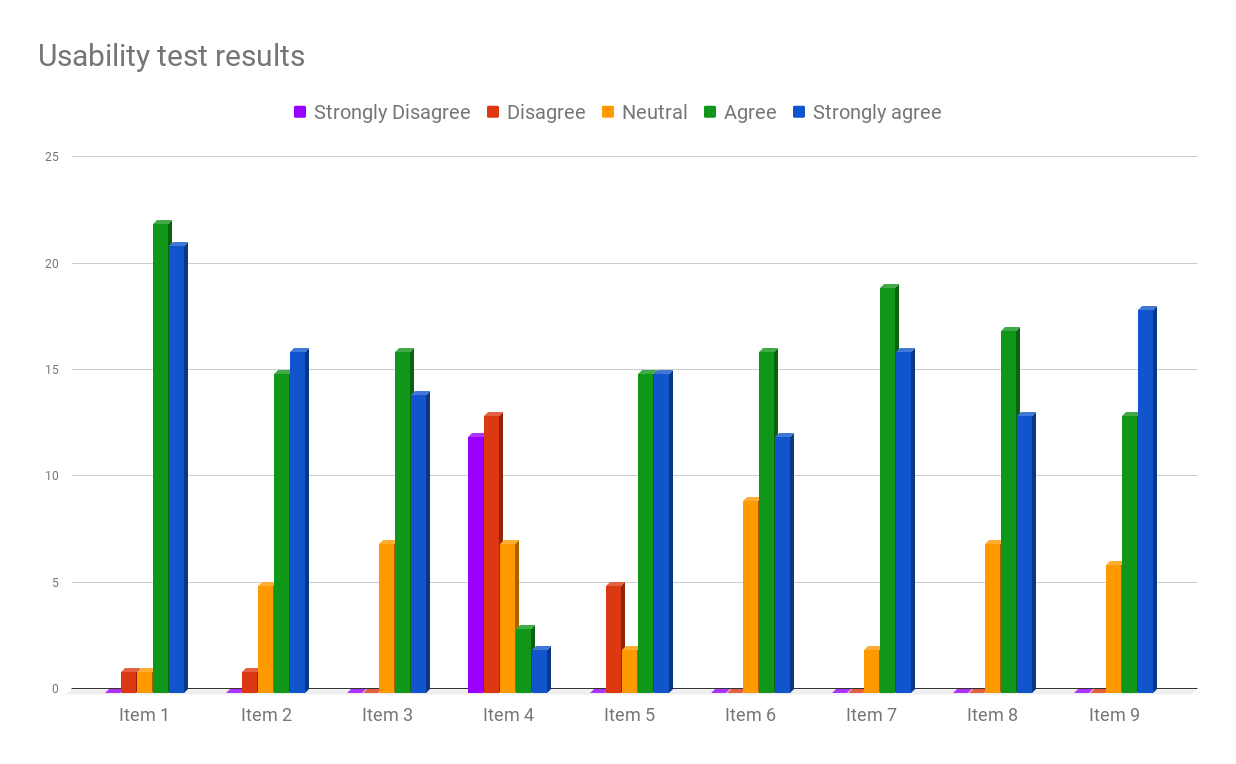
\includegraphics[width=\textwidth]{chart_all.png}
\end{figure}

The first survey item, \textit{"The chatbot explains its purpose clearly"}, aims to evaluate if the chatbot introduce himself in a way that users can easily understand what the purpose of the chatbot is. With 21 \textit{Strongly agree}, 22 \textit{Agree},1 \textit{Neutral}, 1 \textit{Disagree} and zero \textit{Strongly Disagree} responses, results confirms the item statement.

The purpose of the second item, \textit{"During the conversation, the chatbot explains clearly what the user can do"}, is to evaluate if users can easily understand what options the bot makes available to them i.e., what users can do during the various steps of the conversation. The results reveal that 16 participants responded with \textit{Strongly agree}, 15 with \textit{Agree}, 5 with \textit{Neutral}, only 1 with \textit{Disagree} and zero with \textit{Strongly disagree}. It can be said that user available options during the chat are fairly clear.

The third item, \textit{"The onboarding message (the initial greetings) makes you want to continue"}, has the goal to measure the engagement power of the onboarding message. Results are quite positive with 14 \textit{Strongly agree}, 16 \textit{Agree}, 7 \textit{Neutral}, zero \textit{Disagree} and zero \textit{Strongly disagree} responses. The message do its job but it also leaves space for future improvements.

The object of the fourth item, \textit{"The login system that involves the use of an external website is complicated"}, is to see if users finds the login system, which I consider as the weak point of the application, complicated. Surprisingly, results shows that the procedure is well built from a usability perspective, and the majority of users did not find it particularly cumbersome. Response numbers are 2 \textit{Strongly agree}, 3 \textit{Agree}, 7 \textit{Neutral}, 13 \textit{Disagree} and 12 \textit{Strongly disagree}. A note on this item: some users did not understand that the statement had a negative meaning and the answers had to be given backwards from the other items.

The fifth item whose statement is \textit{"It is clear what the external web site does"}, has the goal to understand if the bot explains clearly what is the role of the external website in the login procedure and if the website itself is built is a way that doesn't confuse the user during the experience. This item, together with the fourth, serves to understand the impact on usability of the particular access system due to the multi-platform nature of the bot. The results shows a number of responses of 15 for both \textit{Strongly agree} and \textit{Agree}, 2 for \textit{Neutral}, 5 for \textit{Disagree} and zero for \textit{Strongly disagree}. The outcome can be interpreted as positive because, even if there are 5 \textit{Disagree} responses, the two positive responses marks a triple score.

Item number six, \textit{How do you judge the usefulness of the recommendations?} is an explicit request to users to evaluate the quality of the recommendations in terms of usefulness, that is the actual approval of the recommended artists. Although positive responses score 12 for \textit{Strongly Agree} and 16 for \textit{Agree}, the results show a significant number of \textit{Neutral} responses, 9 to be precise; the reasons for this result are due to the fact that many users did not know the artists proposed and responded to the survey without first having listened to them. Unfortunately, this phenomenon has been difficult to control, but despite this, the overall result is positive.

Regarding the seventh item, \textit{How do you judge the overall experience?}, result are quite positive with a total of 16 \textit{Strongly agree} responses, 19 \textit{Agree} responses, only 2 \textit{Neutral} and zero responses for \textit{Disagree} and \textit{Strongly disagree}. This is a clear sign of the goodness of Beat in a Bot it terms of usability.

The eighth item, \textit{Would you use it again?}, aims to measure if users feels satisfied of the overall experience and consider Beat in a Bot, a valid tool for the recommendation of new music artists to listen to. Results are, no negative responses (\textit{Strongly disagree} and \textit{Disagree}), 7 \textit{Neutral}, 17 \textit{Agree} and 13 \textit{Strongly agree}, showing a good level of user appreciation.

The last item, \textit{Would you recommend it to your friends?}, together with the eighth, wants to evaluate the application as a whole and to check if it is good enough to make people talk about it. An high number of \textit{Strongly agree} and \textit{Agree} responses, 18 and 13 respectively, confirms that the bot has aroused curiosity between users and the 6 \textit{Neutral} responses are an incentive for a further improvement of the service. 

\section{Usefulness test}

The usefulness test, carried out together with the usability test, aims to implicitly measure how much users have found the tool useful, from the number of the positive-only feedback given to the proposed recommendations. Participants were asked to use the bot, scroll through an arbitrary number of suggestions and mark those considered interesting. The actual users of the application were 27, 4 women and 23 men aged between 20 and 35. The distribution of users based on their belonging to a certain Myers-Briggs Type Indicator is shown in the following graph:

\begin{figure}[ht]
\centering
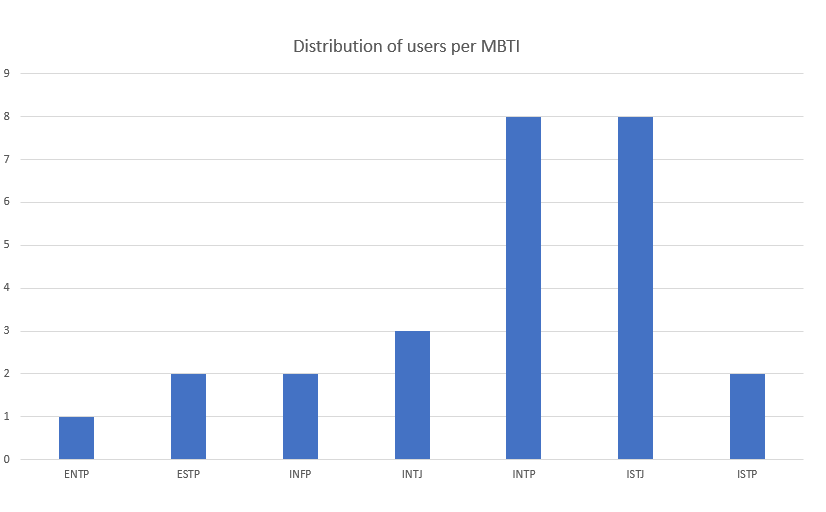
\includegraphics[width=\textwidth]{users_per_MBTI.png}
\end{figure}

Bars indicates a distribution of 8 INTP users, 8 ISTJ users, 3 INTJ users, 2 INFP, 2, ISTP, 2 ESTP, and 1 ENTP user. Adding the feedback from users belonging to the same MBTI group, we obtain a result of 47 feedback from INTP users, 52 feedback from ISTJ users, 33 feedback from INTJ, 14 feedback from INFP, 10 feedback from ISTP, 7 feedback from ESTP and 4 from ENTP. The result is summarized in figure 5.3. Bars indicates the total number of feedback given by each group of users. The similarity between the distribution of users graph and the total number of feedback graph, shows that the number of preferences is directly proportional to the number of users and that the average number of preferences given for each user within his group is similar among the various groups.

\pagebreak
\begin{figure}[ht]
\centering
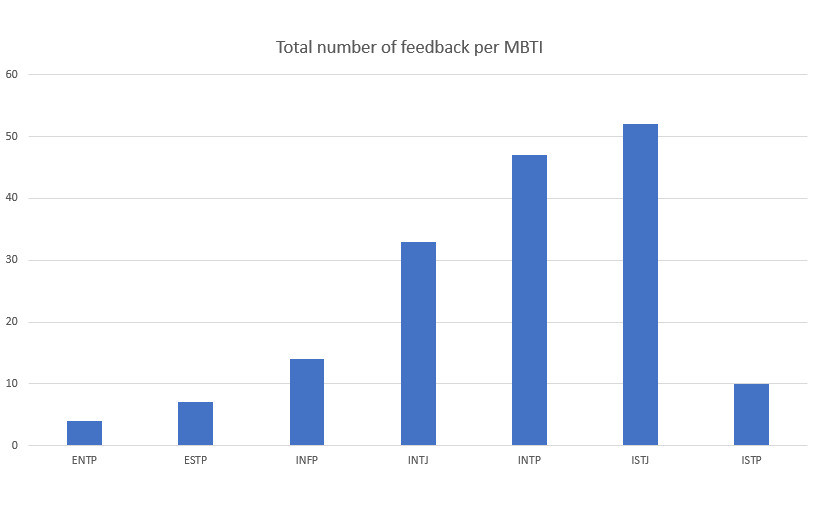
\includegraphics[scale=0.5]{feedback_per_MBTI.png}
\end{figure}

This is clearly shown by the dimension likeness of the coloured part of the radial graph above, where each of them represents the average number of feedback given by users of each group. Numbers are, 5.9 for INTP users, 4 for ENTP users, 3.5 for ESTP users, 7 for INFP, 11 for INTJ, 6.5 for ISTJ and 5 for ISTP. We can conclude that, since the bot gives 16 recommendations for each users and they had the freedom of withdraw at each moment, a number of average feedback greater than 5 for the majority of the group is a good result in terms of application usefulness.    

\begin{figure}[ht]
\centering
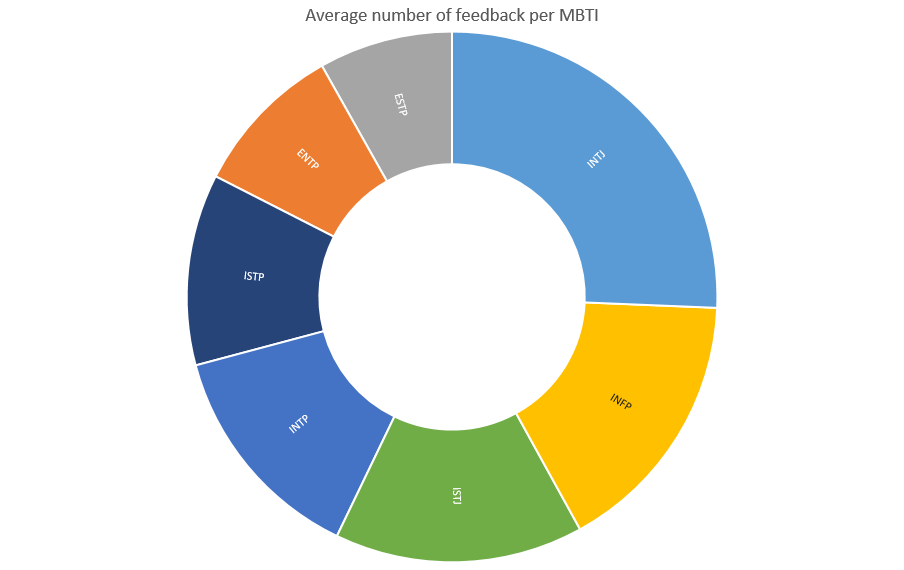
\includegraphics[scale=0.4]{average.png}
\end{figure}


\chapter{Conclusion}

The goal of this project was to experiment chatbots as interface for recommender systems and affective computing. The results of the utility and usefulness test, clearly shows users appreciation for such type of application.

The developed chatbot lends itself to a variety of future improvements. The main one concerns the prediction phase of user's personality. At the moment, it relies upon two external web services, Apply Magic Sauce and Facebook Graph and has the user requirement of a Facebook account. External web services provides a fast and easy way to obtain a result, but they may become a problem for the application maintaining, due to the fact that their functionality may change over time, they have limitations and they are not under the complete control of the chatbot developer. The Facebook account requirement can be an obstacle for privacy concerned people that don't want to share their personal information and also for people that do not have a Facebook account. A solution to this problem is represented by the possibility of predicting the user's personality from the chat itself, using the chat text. This can be achievable expanding the onboarding experience with a little conversation before moving to artist recommendations. There are several products already available that are able to find user's personality from written text, like IBM Personality Insights, Apply Magic Sauce itself and Textgain but, while they eliminates the need of a social account, they still have all the problem of external services. Furthermore, to generate a reliable personality prediction, 100 to 200 words are required and this is difficult to achieve in a chatbot application.

%%% cita il lavoro di ISMB e Giulio Carducci(?)

From a financial perspective, the chatbot can be used to generate earnings applying a freemium business model. Freemium is a pricing strategy by which a product or service is provided free of charge, but money (premium) is charged for additional features, services, or virtual goods   \citep{freemium}. An additional feature may be the possibility of proposing personalized music playlists to users, composed of the best songs by the recommended artists. Playlists can be created for all the different music streaming platforms available, so that the chatbot can be used by a wider audience, rather than being proposed as an individual service.
\\
\\
To conclude, I can say that chatbots, placing themselves in a broader perspective of improvement of human-computer interfaces, certainly represent a valid tool for interacting with users and occupy a place of relevance in the world of modern computer science, increasingly focused on mobile. They represent a good alternative to websites and apps and are flexible enough to be used in conjuction with artificial intelligence, data science, recommender systems and other fields of technology, allowing them to be used in a large variety of applications, from entertaiment, to customer support, from e-commerce to psycho-therapy. 

\bibliographystyle{agsm}
\bibliography{mybib}


\end{document}
